\documentclass[twoside]{book}

% Packages required by doxygen
\usepackage{fixltx2e}
\usepackage{calc}
\usepackage{doxygen}
\usepackage[export]{adjustbox} % also loads graphicx
\usepackage{graphicx}
\usepackage[utf8]{inputenc}
\usepackage{makeidx}
\usepackage{multicol}
\usepackage{multirow}
\PassOptionsToPackage{warn}{textcomp}
\usepackage{textcomp}
\usepackage[nointegrals]{wasysym}
\usepackage[table]{xcolor}

% Font selection
\usepackage[T1]{fontenc}
\usepackage[scaled=.90]{helvet}
\usepackage{courier}
\usepackage{amssymb}
\usepackage{sectsty}
\renewcommand{\familydefault}{\sfdefault}
\allsectionsfont{%
  \fontseries{bc}\selectfont%
  \color{darkgray}%
}
\renewcommand{\DoxyLabelFont}{%
  \fontseries{bc}\selectfont%
  \color{darkgray}%
}
\newcommand{\+}{\discretionary{\mbox{\scriptsize$\hookleftarrow$}}{}{}}

% Page & text layout
\usepackage{geometry}
\geometry{%
  a4paper,%
  top=2.5cm,%
  bottom=2.5cm,%
  left=2.5cm,%
  right=2.5cm%
}
\tolerance=750
\hfuzz=15pt
\hbadness=750
\setlength{\emergencystretch}{15pt}
\setlength{\parindent}{0cm}
\setlength{\parskip}{3ex plus 2ex minus 2ex}
\makeatletter
\renewcommand{\paragraph}{%
  \@startsection{paragraph}{4}{0ex}{-1.0ex}{1.0ex}{%
    \normalfont\normalsize\bfseries\SS@parafont%
  }%
}
\renewcommand{\subparagraph}{%
  \@startsection{subparagraph}{5}{0ex}{-1.0ex}{1.0ex}{%
    \normalfont\normalsize\bfseries\SS@subparafont%
  }%
}
\makeatother

% Headers & footers
\usepackage{fancyhdr}
\pagestyle{fancyplain}
\fancyhead[LE]{\fancyplain{}{\bfseries\thepage}}
\fancyhead[CE]{\fancyplain{}{}}
\fancyhead[RE]{\fancyplain{}{\bfseries\leftmark}}
\fancyhead[LO]{\fancyplain{}{\bfseries\rightmark}}
\fancyhead[CO]{\fancyplain{}{}}
\fancyhead[RO]{\fancyplain{}{\bfseries\thepage}}
\fancyfoot[LE]{\fancyplain{}{}}
\fancyfoot[CE]{\fancyplain{}{}}
\fancyfoot[RE]{\fancyplain{}{\bfseries\scriptsize Generated by Doxygen }}
\fancyfoot[LO]{\fancyplain{}{\bfseries\scriptsize Generated by Doxygen }}
\fancyfoot[CO]{\fancyplain{}{}}
\fancyfoot[RO]{\fancyplain{}{}}
\renewcommand{\footrulewidth}{0.4pt}
\renewcommand{\chaptermark}[1]{%
  \markboth{#1}{}%
}
\renewcommand{\sectionmark}[1]{%
  \markright{\thesection\ #1}%
}

% Indices & bibliography
\usepackage{natbib}
\usepackage[titles]{tocloft}
\setcounter{tocdepth}{3}
\setcounter{secnumdepth}{5}
\makeindex

% Hyperlinks (required, but should be loaded last)
\usepackage{ifpdf}
\ifpdf
  \usepackage[pdftex,pagebackref=true]{hyperref}
\else
  \usepackage[ps2pdf,pagebackref=true]{hyperref}
\fi
\hypersetup{%
  colorlinks=true,%
  linkcolor=blue,%
  citecolor=blue,%
  unicode%
}

% Custom commands
\newcommand{\clearemptydoublepage}{%
  \newpage{\pagestyle{empty}\cleardoublepage}%
}

\usepackage{caption}
\captionsetup{labelsep=space,justification=centering,font={bf},singlelinecheck=off,skip=4pt,position=top}

%===== C O N T E N T S =====

\begin{document}

% Titlepage & ToC
\hypersetup{pageanchor=false,
             bookmarksnumbered=true,
             pdfencoding=unicode
            }
\pagenumbering{alph}
\begin{titlepage}
\vspace*{7cm}
\begin{center}%
{\Large project }\\
\vspace*{1cm}
{\large Generated by Doxygen 1.8.13}\\
\end{center}
\end{titlepage}
\clearemptydoublepage
\pagenumbering{roman}
\tableofcontents
\clearemptydoublepage
\pagenumbering{arabic}
\hypersetup{pageanchor=true}

%--- Begin generated contents ---
\chapter{cpp-\/practice-\/and-\/small-\/toys}
\label{md_README}
\Hypertarget{md_README}
practice and small toys 
\chapter{Hierarchical Index}
\section{Class Hierarchy}
This inheritance list is sorted roughly, but not completely, alphabetically\+:\begin{DoxyCompactList}
\item \contentsline{section}{background\+\_\+task}{\pageref{classbackground__task}}{}
\item \contentsline{section}{Binary\+Tree$<$ T $>$}{\pageref{classBinaryTree}}{}
\begin{DoxyCompactList}
\item \contentsline{section}{Linked\+Binary\+Tree$<$ pair$<$ const K, E $>$ $>$}{\pageref{classLinkedBinaryTree}}{}
\begin{DoxyCompactList}
\item \contentsline{section}{Binary\+Search\+Tree$<$ K, E $>$}{\pageref{classBinarySearchTree}}{}
\item \contentsline{section}{Red\+Black\+Tree$<$ K, E $>$}{\pageref{classRedBlackTree}}{}
\end{DoxyCompactList}
\item \contentsline{section}{Linked\+Binary\+Tree$<$ size\+\_\+t $>$}{\pageref{classLinkedBinaryTree}}{}
\item \contentsline{section}{Linked\+Binary\+Tree$<$ std\+:\+:pair$<$ int, T $>$ $>$}{\pageref{classLinkedBinaryTree}}{}
\begin{DoxyCompactList}
\item \contentsline{section}{Max\+Hblt$<$ T $>$}{\pageref{classMaxHblt}}{}
\end{DoxyCompactList}
\end{DoxyCompactList}
\item \contentsline{section}{Binary\+Tree$<$ Bin\+Tree\+Node$<$ T $>$ $>$}{\pageref{classBinaryTree}}{}
\begin{DoxyCompactList}
\item \contentsline{section}{Linked\+Binary\+Tree$<$ T $>$}{\pageref{classLinkedBinaryTree}}{}
\end{DoxyCompactList}
\item \contentsline{section}{Bin\+Tree\+Node$<$ T $>$}{\pageref{structBinTreeNode}}{}
\item \contentsline{section}{Bin\+Tree\+Node$<$ pair$<$ const K, E $>$ $>$}{\pageref{structBinTreeNode}}{}
\item \contentsline{section}{Bin\+Tree\+Node$<$ size\+\_\+t $>$}{\pageref{structBinTreeNode}}{}
\item \contentsline{section}{Bin\+Tree\+Node$<$ std\+:\+:pair$<$ int, T $>$ $>$}{\pageref{structBinTreeNode}}{}
\item \contentsline{section}{B\+S\+Tree$<$ K, E $>$}{\pageref{classBSTree}}{}
\begin{DoxyCompactList}
\item \contentsline{section}{Binary\+Search\+Tree$<$ K, E $>$}{\pageref{classBinarySearchTree}}{}
\end{DoxyCompactList}
\item \contentsline{section}{Client}{\pageref{classClient}}{}
\item \contentsline{section}{cmp$<$ T $>$}{\pageref{classcmp}}{}
\item \contentsline{section}{C\+Redis\+Publisher}{\pageref{classCRedisPublisher}}{}
\item \contentsline{section}{C\+Redis\+Subscriber}{\pageref{classCRedisSubscriber}}{}
\item \contentsline{section}{func}{\pageref{structfunc}}{}
\item \contentsline{section}{graph$<$ T $>$}{\pageref{classgraph}}{}
\begin{DoxyCompactList}
\item \contentsline{section}{Adjacency\+W\+Digraph$<$ T $>$}{\pageref{classAdjacencyWDigraph}}{}
\end{DoxyCompactList}
\item \contentsline{section}{Huffman\+Node$<$ T $>$}{\pageref{structHuffmanNode}}{}
\item \contentsline{section}{iterator$<$ T $>$}{\pageref{classiterator}}{}
\item \contentsline{section}{Linear\+List$<$ T $>$}{\pageref{classLinearList}}{}
\begin{DoxyCompactList}
\item \contentsline{section}{Array\+List$<$ T $>$}{\pageref{classArrayList}}{}
\item \contentsline{section}{Linked\+List$<$ T $>$}{\pageref{classLinkedList}}{}
\item \contentsline{section}{Vector\+List$<$ T $>$}{\pageref{classVectorList}}{}
\end{DoxyCompactList}
\item \contentsline{section}{Link\+Node$<$ T $>$}{\pageref{structLinkNode}}{}
\item \contentsline{section}{Priority\+Queue$<$ T $>$}{\pageref{classPriorityQueue}}{}
\begin{DoxyCompactList}
\item \contentsline{section}{Max\+Hblt$<$ T $>$}{\pageref{classMaxHblt}}{}
\item \contentsline{section}{Max\+Heap$<$ T $>$}{\pageref{classMaxHeap}}{}
\end{DoxyCompactList}
\item \contentsline{section}{Queue$<$ T $>$}{\pageref{classQueue}}{}
\begin{DoxyCompactList}
\item \contentsline{section}{Array\+Queue$<$ T $>$}{\pageref{classArrayQueue}}{}
\end{DoxyCompactList}
\item \contentsline{section}{R\+B\+Tree\+Node$<$ T $>$}{\pageref{structRBTreeNode}}{}
\item \contentsline{section}{R\+B\+Tree\+Node$<$ pair$<$ const K, E $>$ $>$}{\pageref{structRBTreeNode}}{}
\item \contentsline{section}{R\+B\+Tree\+Node$<$ size\+\_\+t $>$}{\pageref{structRBTreeNode}}{}
\item \contentsline{section}{R\+B\+Tree\+Node$<$ std\+:\+:pair$<$ int, T $>$ $>$}{\pageref{structRBTreeNode}}{}
\item \contentsline{section}{Server}{\pageref{classServer}}{}
\item \contentsline{section}{Stack$<$ T $>$}{\pageref{classStack}}{}
\begin{DoxyCompactList}
\item \contentsline{section}{Array\+Stack$<$ T $>$}{\pageref{classArrayStack}}{}
\item \contentsline{section}{Linked\+Stack$<$ T $>$}{\pageref{classLinkedStack}}{}
\end{DoxyCompactList}
\item \contentsline{section}{vertex\+\_\+iterator$<$ T $>$}{\pageref{classvertex__iterator}}{}
\begin{DoxyCompactList}
\item \contentsline{section}{My\+Iterator$<$ T $>$}{\pageref{classMyIterator}}{}
\end{DoxyCompactList}
\item \contentsline{section}{Winner\+Tree$<$ T $>$}{\pageref{classWinnerTree}}{}
\begin{DoxyCompactList}
\item \contentsline{section}{Complete\+Winner\+Tree$<$ T $>$}{\pageref{classCompleteWinnerTree}}{}
\end{DoxyCompactList}
\end{DoxyCompactList}

\chapter{Class Index}
\section{Class List}
Here are the classes, structs, unions and interfaces with brief descriptions\+:\begin{DoxyCompactList}
\item\contentsline{section}{\hyperlink{classAdjacencyWDigraph}{Adjacency\+W\+Digraph$<$ T $>$} }{\pageref{classAdjacencyWDigraph}}{}
\item\contentsline{section}{\hyperlink{classArrayList}{Array\+List$<$ T $>$} }{\pageref{classArrayList}}{}
\item\contentsline{section}{\hyperlink{classArrayQueue}{Array\+Queue$<$ T $>$} }{\pageref{classArrayQueue}}{}
\item\contentsline{section}{\hyperlink{classArrayStack}{Array\+Stack$<$ T $>$} }{\pageref{classArrayStack}}{}
\item\contentsline{section}{\hyperlink{classbackground__task}{background\+\_\+task} }{\pageref{classbackground__task}}{}
\item\contentsline{section}{\hyperlink{classBinarySearchTree}{Binary\+Search\+Tree$<$ K, E $>$} }{\pageref{classBinarySearchTree}}{}
\item\contentsline{section}{\hyperlink{classBinaryTree}{Binary\+Tree$<$ T $>$} }{\pageref{classBinaryTree}}{}
\item\contentsline{section}{\hyperlink{structBinTreeNode}{Bin\+Tree\+Node$<$ T $>$} }{\pageref{structBinTreeNode}}{}
\item\contentsline{section}{\hyperlink{classBSTree}{B\+S\+Tree$<$ K, E $>$} }{\pageref{classBSTree}}{}
\item\contentsline{section}{\hyperlink{classClient}{Client} }{\pageref{classClient}}{}
\item\contentsline{section}{\hyperlink{classcmp}{cmp$<$ T $>$} }{\pageref{classcmp}}{}
\item\contentsline{section}{\hyperlink{classCompleteWinnerTree}{Complete\+Winner\+Tree$<$ T $>$} }{\pageref{classCompleteWinnerTree}}{}
\item\contentsline{section}{\hyperlink{classCRedisPublisher}{C\+Redis\+Publisher} }{\pageref{classCRedisPublisher}}{}
\item\contentsline{section}{\hyperlink{classCRedisSubscriber}{C\+Redis\+Subscriber} }{\pageref{classCRedisSubscriber}}{}
\item\contentsline{section}{\hyperlink{structfunc}{func} }{\pageref{structfunc}}{}
\item\contentsline{section}{\hyperlink{classgraph}{graph$<$ T $>$} }{\pageref{classgraph}}{}
\item\contentsline{section}{\hyperlink{structHuffmanNode}{Huffman\+Node$<$ T $>$} }{\pageref{structHuffmanNode}}{}
\item\contentsline{section}{\hyperlink{classiterator}{iterator$<$ T $>$} }{\pageref{classiterator}}{}
\item\contentsline{section}{\hyperlink{classLinearList}{Linear\+List$<$ T $>$} }{\pageref{classLinearList}}{}
\item\contentsline{section}{\hyperlink{classLinkedBinaryTree}{Linked\+Binary\+Tree$<$ T $>$} }{\pageref{classLinkedBinaryTree}}{}
\item\contentsline{section}{\hyperlink{classLinkedList}{Linked\+List$<$ T $>$} }{\pageref{classLinkedList}}{}
\item\contentsline{section}{\hyperlink{classLinkedStack}{Linked\+Stack$<$ T $>$} }{\pageref{classLinkedStack}}{}
\item\contentsline{section}{\hyperlink{structLinkNode}{Link\+Node$<$ T $>$} }{\pageref{structLinkNode}}{}
\item\contentsline{section}{\hyperlink{classMaxHblt}{Max\+Hblt$<$ T $>$} }{\pageref{classMaxHblt}}{}
\item\contentsline{section}{\hyperlink{classMaxHeap}{Max\+Heap$<$ T $>$} }{\pageref{classMaxHeap}}{}
\item\contentsline{section}{\hyperlink{classMyIterator}{My\+Iterator$<$ T $>$} }{\pageref{classMyIterator}}{}
\item\contentsline{section}{\hyperlink{classPriorityQueue}{Priority\+Queue$<$ T $>$} }{\pageref{classPriorityQueue}}{}
\item\contentsline{section}{\hyperlink{classQueue}{Queue$<$ T $>$} }{\pageref{classQueue}}{}
\item\contentsline{section}{\hyperlink{structRBTreeNode}{R\+B\+Tree\+Node$<$ T $>$} }{\pageref{structRBTreeNode}}{}
\item\contentsline{section}{\hyperlink{classRedBlackTree}{Red\+Black\+Tree$<$ K, E $>$} }{\pageref{classRedBlackTree}}{}
\item\contentsline{section}{\hyperlink{classServer}{Server} }{\pageref{classServer}}{}
\item\contentsline{section}{\hyperlink{classStack}{Stack$<$ T $>$} }{\pageref{classStack}}{}
\item\contentsline{section}{\hyperlink{classVectorList}{Vector\+List$<$ T $>$} }{\pageref{classVectorList}}{}
\item\contentsline{section}{\hyperlink{classvertex__iterator}{vertex\+\_\+iterator$<$ T $>$} }{\pageref{classvertex__iterator}}{}
\item\contentsline{section}{\hyperlink{classWinnerTree}{Winner\+Tree$<$ T $>$} }{\pageref{classWinnerTree}}{}
\end{DoxyCompactList}

\chapter{Class Documentation}
\hypertarget{classAdjacencyWDigraph}{}\section{Adjacency\+W\+Digraph$<$ T $>$ Class Template Reference}
\label{classAdjacencyWDigraph}\index{Adjacency\+W\+Digraph$<$ T $>$@{Adjacency\+W\+Digraph$<$ T $>$}}
Inheritance diagram for Adjacency\+W\+Digraph$<$ T $>$\+:\begin{figure}[H]
\begin{center}
\leavevmode
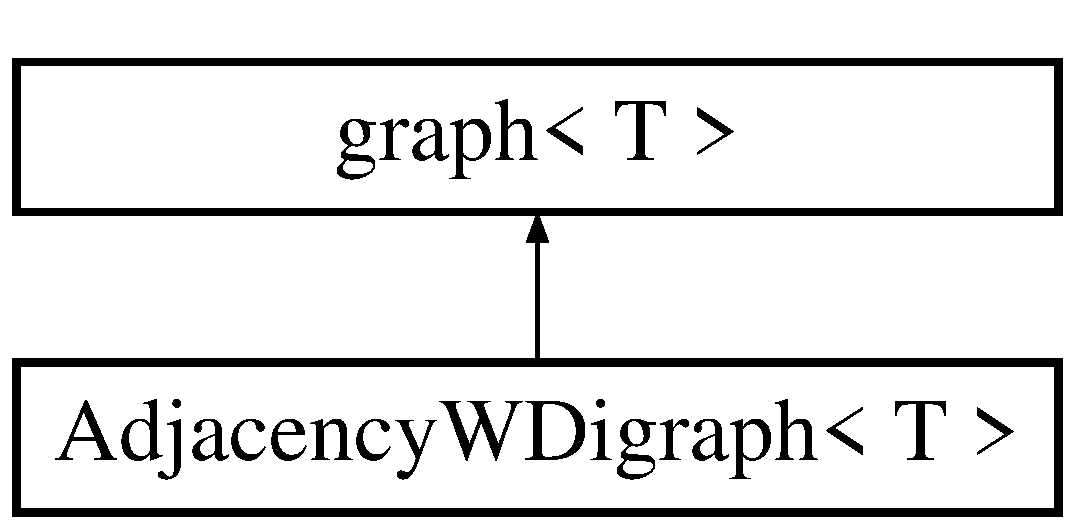
\includegraphics[height=2.000000cm]{classAdjacencyWDigraph}
\end{center}
\end{figure}
\subsection*{Public Member Functions}
\begin{DoxyCompactItemize}
\item 
\mbox{\Hypertarget{classAdjacencyWDigraph_aba0b8944172c501a75e4ceb4ce6de298}\label{classAdjacencyWDigraph_aba0b8944172c501a75e4ceb4ce6de298}} 
{\bfseries Adjacency\+W\+Digraph} (int num\+\_\+of\+\_\+vertices=0, T the\+\_\+no\+\_\+edges=0)
\item 
\mbox{\Hypertarget{classAdjacencyWDigraph_ac5fe40a92fd523e38556074638ebb0d9}\label{classAdjacencyWDigraph_ac5fe40a92fd523e38556074638ebb0d9}} 
int {\bfseries num\+\_\+of\+\_\+vertices} () const
\item 
\mbox{\Hypertarget{classAdjacencyWDigraph_a1f7c91568a37048136fbeaa745198342}\label{classAdjacencyWDigraph_a1f7c91568a37048136fbeaa745198342}} 
int {\bfseries num\+\_\+of\+\_\+edges} () const
\item 
\mbox{\Hypertarget{classAdjacencyWDigraph_a2798e841423506f8c269758a945f33ca}\label{classAdjacencyWDigraph_a2798e841423506f8c269758a945f33ca}} 
bool {\bfseries exists\+\_\+edge} (int, int) const
\item 
\mbox{\Hypertarget{classAdjacencyWDigraph_a1f1f40e28e3560a9acef4a570c805d2e}\label{classAdjacencyWDigraph_a1f1f40e28e3560a9acef4a570c805d2e}} 
void {\bfseries insert\+\_\+edge} (int, int, T)
\item 
\mbox{\Hypertarget{classAdjacencyWDigraph_a35b3e083122c98bd9095a4ec2fab569d}\label{classAdjacencyWDigraph_a35b3e083122c98bd9095a4ec2fab569d}} 
void {\bfseries erase\+\_\+edge} (int, int)
\item 
\mbox{\Hypertarget{classAdjacencyWDigraph_a1765659ef5b2a3ba21f1427070a2047c}\label{classAdjacencyWDigraph_a1765659ef5b2a3ba21f1427070a2047c}} 
bool {\bfseries check\+\_\+vertex} (int the\+\_\+vertex) const
\item 
\mbox{\Hypertarget{classAdjacencyWDigraph_ac6fc7649a511cba682a0a5ea9dbd8850}\label{classAdjacencyWDigraph_ac6fc7649a511cba682a0a5ea9dbd8850}} 
int {\bfseries degree} (int) const
\item 
\mbox{\Hypertarget{classAdjacencyWDigraph_ab61bb7a2fe0c23439f70d25f93b3943b}\label{classAdjacencyWDigraph_ab61bb7a2fe0c23439f70d25f93b3943b}} 
int {\bfseries in\+\_\+degree} (int) const
\item 
\mbox{\Hypertarget{classAdjacencyWDigraph_ab33938596c7dfeec5830dd9e3ea33ce1}\label{classAdjacencyWDigraph_ab33938596c7dfeec5830dd9e3ea33ce1}} 
int {\bfseries out\+\_\+degree} (int) const
\item 
\mbox{\Hypertarget{classAdjacencyWDigraph_a7a7de2aac4ae34a5a8cbe9c592faed59}\label{classAdjacencyWDigraph_a7a7de2aac4ae34a5a8cbe9c592faed59}} 
bool {\bfseries directed} () const
\item 
\mbox{\Hypertarget{classAdjacencyWDigraph_a6f9db4aec4cefb4c07f6fb26a5ab9c65}\label{classAdjacencyWDigraph_a6f9db4aec4cefb4c07f6fb26a5ab9c65}} 
bool {\bfseries weighted} () const
\item 
\mbox{\Hypertarget{classAdjacencyWDigraph_af9cb59bd782511466f82a011b4f5ad73}\label{classAdjacencyWDigraph_af9cb59bd782511466f82a011b4f5ad73}} 
\hyperlink{classMyIterator}{My\+Iterator}$<$ T $>$ $\ast$ {\bfseries iterator} (int the\+\_\+vertex)
\end{DoxyCompactItemize}
\subsection*{Protected Attributes}
\begin{DoxyCompactItemize}
\item 
\mbox{\Hypertarget{classAdjacencyWDigraph_a37b4dab62f983a0848c62ee4d3b76ee3}\label{classAdjacencyWDigraph_a37b4dab62f983a0848c62ee4d3b76ee3}} 
int {\bfseries n}
\item 
\mbox{\Hypertarget{classAdjacencyWDigraph_a864817f005e567120b21ed296ab56819}\label{classAdjacencyWDigraph_a864817f005e567120b21ed296ab56819}} 
int {\bfseries e}
\item 
\mbox{\Hypertarget{classAdjacencyWDigraph_a7da8b19b024f300504cc2201bc7a0aae}\label{classAdjacencyWDigraph_a7da8b19b024f300504cc2201bc7a0aae}} 
T $\ast$$\ast$ {\bfseries a}
\item 
\mbox{\Hypertarget{classAdjacencyWDigraph_accd1b00deb25b12bb7bf5d57e53218e9}\label{classAdjacencyWDigraph_accd1b00deb25b12bb7bf5d57e53218e9}} 
T {\bfseries no\+\_\+edge}
\end{DoxyCompactItemize}


The documentation for this class was generated from the following file\+:\begin{DoxyCompactItemize}
\item 
data\+\_\+structure/graph/adj\+\_\+wdigraph.\+h\end{DoxyCompactItemize}

\hypertarget{classArrayList}{}\section{Array\+List$<$ T $>$ Class Template Reference}
\label{classArrayList}\index{Array\+List$<$ T $>$@{Array\+List$<$ T $>$}}
Inheritance diagram for Array\+List$<$ T $>$\+:\begin{figure}[H]
\begin{center}
\leavevmode
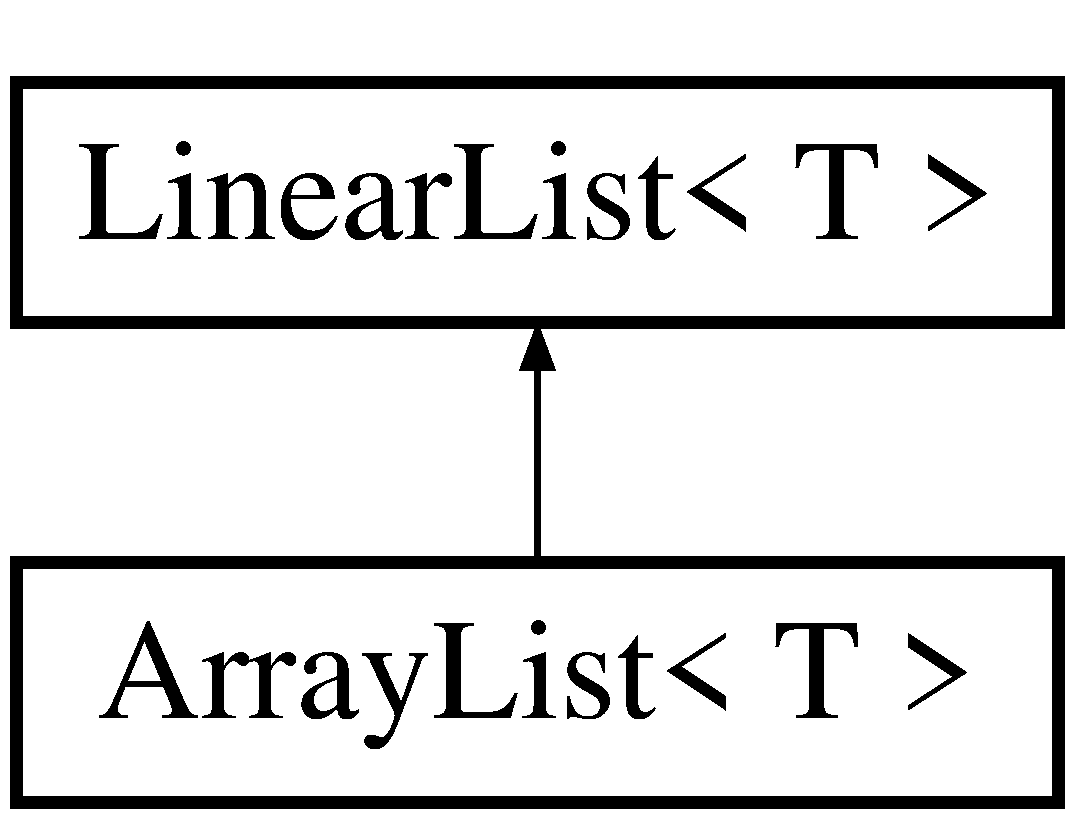
\includegraphics[height=2.000000cm]{classArrayList}
\end{center}
\end{figure}
\subsection*{Public Member Functions}
\begin{DoxyCompactItemize}
\item 
\mbox{\Hypertarget{classArrayList_aa7ccd459591a64ad35d1616c0e69b7c5}\label{classArrayList_aa7ccd459591a64ad35d1616c0e69b7c5}} 
{\bfseries Array\+List} (int length=10)
\item 
\mbox{\Hypertarget{classArrayList_a74e263c5124033910728983d31fc151f}\label{classArrayList_a74e263c5124033910728983d31fc151f}} 
{\bfseries Array\+List} (const \hyperlink{classArrayList}{Array\+List}$<$ T $>$ \&)
\item 
\mbox{\Hypertarget{classArrayList_a3da2b90afa063750438ddc77e178ce24}\label{classArrayList_a3da2b90afa063750438ddc77e178ce24}} 
bool {\bfseries empty} () const
\item 
\mbox{\Hypertarget{classArrayList_ae4b736366ef526783e473ae6dd372f1c}\label{classArrayList_ae4b736366ef526783e473ae6dd372f1c}} 
int {\bfseries size} () const
\item 
\mbox{\Hypertarget{classArrayList_ac777ab7e5967cf10b2a7df72dfbb914d}\label{classArrayList_ac777ab7e5967cf10b2a7df72dfbb914d}} 
T \& {\bfseries get} (int the\+Index) const
\item 
\mbox{\Hypertarget{classArrayList_a30daf5cbd355d72a6d957b8436233aa3}\label{classArrayList_a30daf5cbd355d72a6d957b8436233aa3}} 
int {\bfseries index\+Of} (const T \&the\+Element) const
\item 
\mbox{\Hypertarget{classArrayList_a40123979eb1b36d3e35aa108be3eecd3}\label{classArrayList_a40123979eb1b36d3e35aa108be3eecd3}} 
void {\bfseries erase} (int the\+Index)
\item 
\mbox{\Hypertarget{classArrayList_a58663cbe645ff5075865bca1917792be}\label{classArrayList_a58663cbe645ff5075865bca1917792be}} 
void {\bfseries insert} (int the\+Index, const T \&the\+Element)
\item 
\mbox{\Hypertarget{classArrayList_ac53a6082c9b8cdbceafb0e9675a0999b}\label{classArrayList_ac53a6082c9b8cdbceafb0e9675a0999b}} 
void {\bfseries output} (std\+::ostream \&out) const
\item 
\mbox{\Hypertarget{classArrayList_a8cdac6b82bb2435e33028a16b951d43c}\label{classArrayList_a8cdac6b82bb2435e33028a16b951d43c}} 
void {\bfseries push\+\_\+back} (const T \&the\+Element)
\item 
\mbox{\Hypertarget{classArrayList_a1bfa082439cbecf0e563996e3a10811f}\label{classArrayList_a1bfa082439cbecf0e563996e3a10811f}} 
\hyperlink{classiterator}{iterator}$<$ T $>$ {\bfseries begin} ()
\item 
\mbox{\Hypertarget{classArrayList_ae0f652b027f113a5de5e8e1e6cb81d5b}\label{classArrayList_ae0f652b027f113a5de5e8e1e6cb81d5b}} 
\hyperlink{classiterator}{iterator}$<$ T $>$ {\bfseries end} ()
\end{DoxyCompactItemize}
\subsection*{Protected Member Functions}
\begin{DoxyCompactItemize}
\item 
\mbox{\Hypertarget{classArrayList_a021f10fc94b16d6c6aea82ea11c0be5c}\label{classArrayList_a021f10fc94b16d6c6aea82ea11c0be5c}} 
void {\bfseries check\+Index} (int the\+Index) const
\end{DoxyCompactItemize}
\subsection*{Protected Attributes}
\begin{DoxyCompactItemize}
\item 
\mbox{\Hypertarget{classArrayList_a8770fb8b423372b9747b52058eeb4a1d}\label{classArrayList_a8770fb8b423372b9747b52058eeb4a1d}} 
T $\ast$ {\bfseries element}
\item 
\mbox{\Hypertarget{classArrayList_a619f07a2d43b7eb8443aab9cb268be11}\label{classArrayList_a619f07a2d43b7eb8443aab9cb268be11}} 
int {\bfseries length}
\item 
\mbox{\Hypertarget{classArrayList_a9c205a059f9bdb42fe12cf9f63671a7c}\label{classArrayList_a9c205a059f9bdb42fe12cf9f63671a7c}} 
int {\bfseries list\+\_\+size}
\end{DoxyCompactItemize}


The documentation for this class was generated from the following file\+:\begin{DoxyCompactItemize}
\item 
data\+\_\+structure/linear\+\_\+list/array\+\_\+list.\+h\end{DoxyCompactItemize}

\hypertarget{classArrayQueue}{}\section{Array\+Queue$<$ T $>$ Class Template Reference}
\label{classArrayQueue}\index{Array\+Queue$<$ T $>$@{Array\+Queue$<$ T $>$}}
Inheritance diagram for Array\+Queue$<$ T $>$\+:\begin{figure}[H]
\begin{center}
\leavevmode
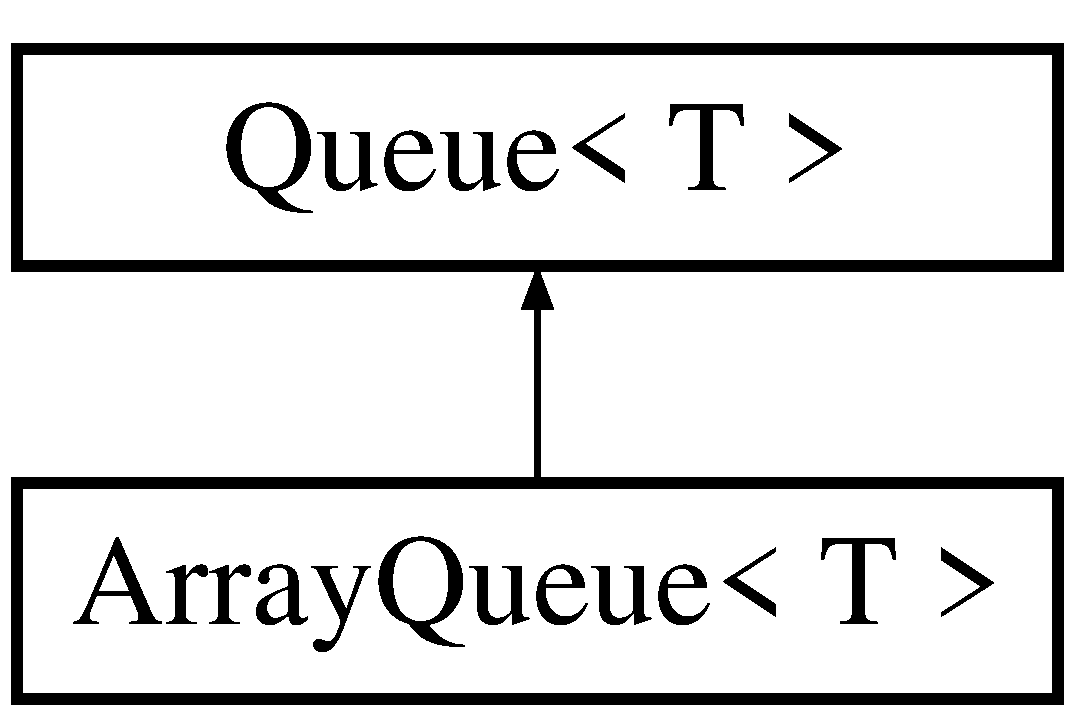
\includegraphics[height=2.000000cm]{classArrayQueue}
\end{center}
\end{figure}
\subsection*{Public Member Functions}
\begin{DoxyCompactItemize}
\item 
\mbox{\Hypertarget{classArrayQueue_ab5b514bd3a1b12782349b4780c5a857e}\label{classArrayQueue_ab5b514bd3a1b12782349b4780c5a857e}} 
{\bfseries Array\+Queue} (const \hyperlink{classArrayQueue}{Array\+Queue}$<$ T $>$ \&)
\item 
\mbox{\Hypertarget{classArrayQueue_a2781468de08c00f8f5fb4ccc1485605a}\label{classArrayQueue_a2781468de08c00f8f5fb4ccc1485605a}} 
bool {\bfseries empty} () const
\item 
\mbox{\Hypertarget{classArrayQueue_ae75aad860a1c25ddb43945365d0ecfe1}\label{classArrayQueue_ae75aad860a1c25ddb43945365d0ecfe1}} 
int {\bfseries size} () const
\item 
\mbox{\Hypertarget{classArrayQueue_ad9be350fa69111973f9adc1f357330e6}\label{classArrayQueue_ad9be350fa69111973f9adc1f357330e6}} 
T \& {\bfseries front} ()
\item 
\mbox{\Hypertarget{classArrayQueue_a98b5d50c5b7c8f9ae342bb1a4b39f1ad}\label{classArrayQueue_a98b5d50c5b7c8f9ae342bb1a4b39f1ad}} 
T \& {\bfseries back} ()
\item 
\mbox{\Hypertarget{classArrayQueue_a2963c72eb08fea6a71561ad2b50cacab}\label{classArrayQueue_a2963c72eb08fea6a71561ad2b50cacab}} 
T {\bfseries pop} ()
\item 
\mbox{\Hypertarget{classArrayQueue_a47169b6217833d23957a5d34f72cdb2b}\label{classArrayQueue_a47169b6217833d23957a5d34f72cdb2b}} 
void {\bfseries push} (const T \&element)
\item 
\mbox{\Hypertarget{classArrayQueue_a266966b8e1d1ec4f9086194df996a1d4}\label{classArrayQueue_a266966b8e1d1ec4f9086194df996a1d4}} 
void {\bfseries output} (std\+::ostream \&out) const
\end{DoxyCompactItemize}
\subsection*{Private Member Functions}
\begin{DoxyCompactItemize}
\item 
\mbox{\Hypertarget{classArrayQueue_ab7696081f60af4fe1aab9c607c0c6c5e}\label{classArrayQueue_ab7696081f60af4fe1aab9c607c0c6c5e}} 
int {\bfseries convert} (int i) const
\item 
\mbox{\Hypertarget{classArrayQueue_a965b1f57a75434cd6bbfeb6ef792a999}\label{classArrayQueue_a965b1f57a75434cd6bbfeb6ef792a999}} 
void {\bfseries change\+\_\+length} ()
\end{DoxyCompactItemize}
\subsection*{Private Attributes}
\begin{DoxyCompactItemize}
\item 
\mbox{\Hypertarget{classArrayQueue_a1fcffdd9b49b218176a4abcb79fbf210}\label{classArrayQueue_a1fcffdd9b49b218176a4abcb79fbf210}} 
T $\ast$ {\bfseries queue}
\item 
\mbox{\Hypertarget{classArrayQueue_a2b8c600fa5f0d1f7d427de65c89c30e2}\label{classArrayQueue_a2b8c600fa5f0d1f7d427de65c89c30e2}} 
int {\bfseries qfront}
\item 
\mbox{\Hypertarget{classArrayQueue_a579a67f77e917054484beb9e4b0d70ee}\label{classArrayQueue_a579a67f77e917054484beb9e4b0d70ee}} 
int {\bfseries qback}
\item 
\mbox{\Hypertarget{classArrayQueue_afaedf9018ab60ddfc5cbe6f8334a33cd}\label{classArrayQueue_afaedf9018ab60ddfc5cbe6f8334a33cd}} 
int {\bfseries queue\+\_\+size}
\end{DoxyCompactItemize}


The documentation for this class was generated from the following file\+:\begin{DoxyCompactItemize}
\item 
data\+\_\+structure/queue/array\+\_\+queue.\+h\end{DoxyCompactItemize}

\hypertarget{classArrayStack}{}\section{Array\+Stack$<$ T $>$ Class Template Reference}
\label{classArrayStack}\index{Array\+Stack$<$ T $>$@{Array\+Stack$<$ T $>$}}
Inheritance diagram for Array\+Stack$<$ T $>$\+:\begin{figure}[H]
\begin{center}
\leavevmode
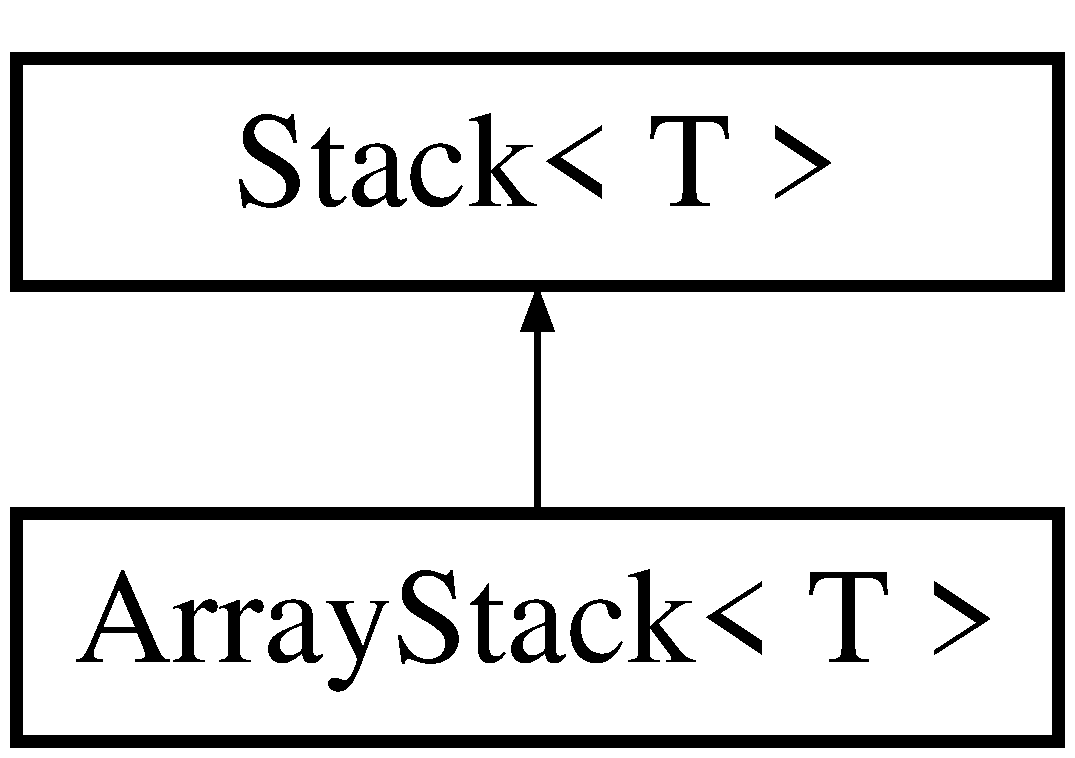
\includegraphics[height=2.000000cm]{classArrayStack}
\end{center}
\end{figure}
\subsection*{Public Member Functions}
\begin{DoxyCompactItemize}
\item 
\mbox{\Hypertarget{classArrayStack_a3079fd948741fa5856ca36881f5ca81e}\label{classArrayStack_a3079fd948741fa5856ca36881f5ca81e}} 
{\bfseries Array\+Stack} (int length=10)
\item 
\mbox{\Hypertarget{classArrayStack_a29471ad4a3d1dfeb388e89e733c41b3b}\label{classArrayStack_a29471ad4a3d1dfeb388e89e733c41b3b}} 
bool {\bfseries empty} () const
\item 
\mbox{\Hypertarget{classArrayStack_aab54ac6bfa973f73114e3bd110257893}\label{classArrayStack_aab54ac6bfa973f73114e3bd110257893}} 
int {\bfseries size} () const
\item 
\mbox{\Hypertarget{classArrayStack_ad5486caf1345bbe1abeb5a154ee3a54e}\label{classArrayStack_ad5486caf1345bbe1abeb5a154ee3a54e}} 
T {\bfseries pop} ()
\item 
\mbox{\Hypertarget{classArrayStack_abec8b059a99c03f85e8e78fc3a5e4c5b}\label{classArrayStack_abec8b059a99c03f85e8e78fc3a5e4c5b}} 
void {\bfseries push} (const T \&element)
\item 
\mbox{\Hypertarget{classArrayStack_aec6eac3f779260b173210794b2d55b04}\label{classArrayStack_aec6eac3f779260b173210794b2d55b04}} 
void {\bfseries output} (std\+::ostream \&out) const
\end{DoxyCompactItemize}
\subsection*{Private Attributes}
\begin{DoxyCompactItemize}
\item 
\mbox{\Hypertarget{classArrayStack_ae828e7a9c71bb3fddf0dd5630cc46565}\label{classArrayStack_ae828e7a9c71bb3fddf0dd5630cc46565}} 
int {\bfseries top}
\item 
\mbox{\Hypertarget{classArrayStack_a8a6aa843f59c9c06660b5b523835456a}\label{classArrayStack_a8a6aa843f59c9c06660b5b523835456a}} 
int {\bfseries length}
\item 
\mbox{\Hypertarget{classArrayStack_a0014804227d2de0343475323939e1518}\label{classArrayStack_a0014804227d2de0343475323939e1518}} 
T $\ast$ {\bfseries stack}
\end{DoxyCompactItemize}


The documentation for this class was generated from the following file\+:\begin{DoxyCompactItemize}
\item 
data\+\_\+structure/stack/Array\+Stack.\+h\end{DoxyCompactItemize}

\hypertarget{classbackground__task}{}\section{background\+\_\+task Class Reference}
\label{classbackground__task}\index{background\+\_\+task@{background\+\_\+task}}
\subsection*{Public Member Functions}
\begin{DoxyCompactItemize}
\item 
\mbox{\Hypertarget{classbackground__task_a116a774b35cf02ea68022f0be37f2ce9}\label{classbackground__task_a116a774b35cf02ea68022f0be37f2ce9}} 
void {\bfseries operator()} () const
\end{DoxyCompactItemize}


The documentation for this class was generated from the following file\+:\begin{DoxyCompactItemize}
\item 
thread/test\+\_\+temp.\+cc\end{DoxyCompactItemize}

\hypertarget{classBinarySearchTree}{}\section{Binary\+Search\+Tree$<$ K, E $>$ Class Template Reference}
\label{classBinarySearchTree}\index{Binary\+Search\+Tree$<$ K, E $>$@{Binary\+Search\+Tree$<$ K, E $>$}}
Inheritance diagram for Binary\+Search\+Tree$<$ K, E $>$\+:\begin{figure}[H]
\begin{center}
\leavevmode
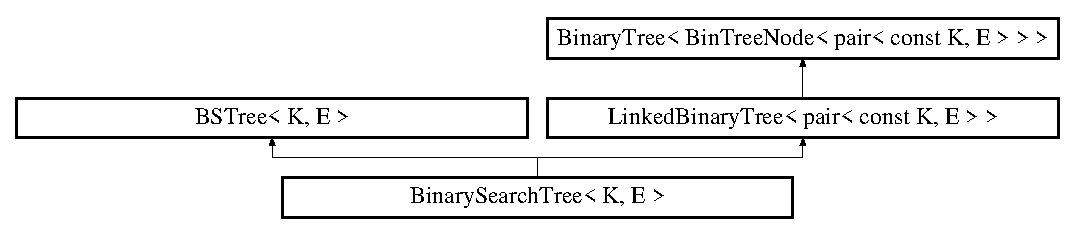
\includegraphics[height=2.700965cm]{classBinarySearchTree}
\end{center}
\end{figure}
\subsection*{Public Member Functions}
\begin{DoxyCompactItemize}
\item 
\mbox{\Hypertarget{classBinarySearchTree_a44aafb261ff5b712be534743cfa88678}\label{classBinarySearchTree_a44aafb261ff5b712be534743cfa88678}} 
const pair$<$ const K, E $>$ {\bfseries find} (const K \&) const
\item 
\mbox{\Hypertarget{classBinarySearchTree_a316a8f1205b0b49bf7e6a49a26d595d9}\label{classBinarySearchTree_a316a8f1205b0b49bf7e6a49a26d595d9}} 
void {\bfseries insert} (const pair$<$ const K, E $>$ \&)
\item 
\mbox{\Hypertarget{classBinarySearchTree_a755fe515b0c387f2e4decee262d08984}\label{classBinarySearchTree_a755fe515b0c387f2e4decee262d08984}} 
void {\bfseries erase} (const K \&)
\item 
\mbox{\Hypertarget{classBinarySearchTree_a637150c98765c148117ed3e96bc90e05}\label{classBinarySearchTree_a637150c98765c148117ed3e96bc90e05}} 
void {\bfseries ascend} ()
\end{DoxyCompactItemize}
\subsection*{Private Member Functions}
\begin{DoxyCompactItemize}
\item 
\mbox{\Hypertarget{classBinarySearchTree_a5a0d9865d5c5c0780f9abc756547a2bc}\label{classBinarySearchTree_a5a0d9865d5c5c0780f9abc756547a2bc}} 
void {\bfseries ascend} (\hyperlink{structBinTreeNode}{Bin\+Tree\+Node}$<$ pair$<$ const K, E $>$$>$ $\ast$)
\end{DoxyCompactItemize}
\subsection*{Additional Inherited Members}


The documentation for this class was generated from the following file\+:\begin{DoxyCompactItemize}
\item 
data\+\_\+structure/tree/binary\+\_\+search\+\_\+tree.\+h\end{DoxyCompactItemize}

\hypertarget{classBinaryTree}{}\section{Binary\+Tree$<$ T $>$ Class Template Reference}
\label{classBinaryTree}\index{Binary\+Tree$<$ T $>$@{Binary\+Tree$<$ T $>$}}
Inheritance diagram for Binary\+Tree$<$ T $>$\+:\begin{figure}[H]
\begin{center}
\leavevmode
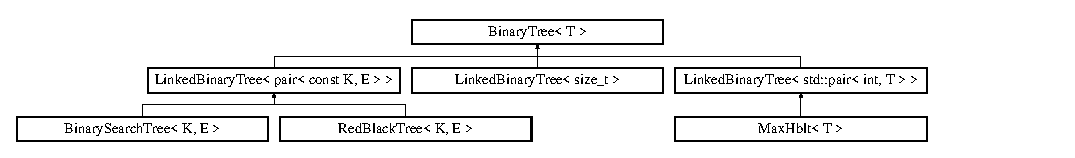
\includegraphics[height=1.680000cm]{classBinaryTree}
\end{center}
\end{figure}
\subsection*{Public Member Functions}
\begin{DoxyCompactItemize}
\item 
\mbox{\Hypertarget{classBinaryTree_a6d3447d1a09fa69e4e34e25f0f53b6f1}\label{classBinaryTree_a6d3447d1a09fa69e4e34e25f0f53b6f1}} 
virtual bool {\bfseries empty} () const =0
\item 
\mbox{\Hypertarget{classBinaryTree_a6f43c6aee330a62beeb0fedb3be25404}\label{classBinaryTree_a6f43c6aee330a62beeb0fedb3be25404}} 
virtual size\+\_\+t {\bfseries size} () const =0
\item 
virtual void \hyperlink{classBinaryTree_a34fabb6ce2424c3ef1e038e148e273c5}{Pre\+Order} (void($\ast$)(T $\ast$))=0
\item 
virtual void \hyperlink{classBinaryTree_a45706a2cafb858f169506470ae440c8a}{In\+Order} (void($\ast$)(T $\ast$))=0
\item 
virtual void \hyperlink{classBinaryTree_a8bc36fb3d3a12ef13d30cc9b4b84e428}{Post\+Order} (void($\ast$)(T $\ast$))=0
\item 
virtual void \hyperlink{classBinaryTree_a1d6ccf7f6b6e1b9a702b12fd5ca6dc32}{Level\+Order} (void($\ast$)(T $\ast$))=0
\end{DoxyCompactItemize}


\subsection{Member Function Documentation}
\mbox{\Hypertarget{classBinaryTree_a45706a2cafb858f169506470ae440c8a}\label{classBinaryTree_a45706a2cafb858f169506470ae440c8a}} 
\index{Binary\+Tree@{Binary\+Tree}!In\+Order@{In\+Order}}
\index{In\+Order@{In\+Order}!Binary\+Tree@{Binary\+Tree}}
\subsubsection{\texorpdfstring{In\+Order()}{InOrder()}}
{\footnotesize\ttfamily template$<$class T$>$ \\
virtual void \hyperlink{classBinaryTree}{Binary\+Tree}$<$ T $>$\+::In\+Order (\begin{DoxyParamCaption}\item[{void($\ast$)(T $\ast$)}]{ }\end{DoxyParamCaption})\hspace{0.3cm}{\ttfamily [pure virtual]}}

visit the tree with inorder \begin{DoxyVerb}left --> root --> right
\end{DoxyVerb}
 

Implemented in \hyperlink{classLinkedBinaryTree_a82b1a5995e90671905da7502d7f58eba}{Linked\+Binary\+Tree$<$ T $>$}.

\mbox{\Hypertarget{classBinaryTree_a1d6ccf7f6b6e1b9a702b12fd5ca6dc32}\label{classBinaryTree_a1d6ccf7f6b6e1b9a702b12fd5ca6dc32}} 
\index{Binary\+Tree@{Binary\+Tree}!Level\+Order@{Level\+Order}}
\index{Level\+Order@{Level\+Order}!Binary\+Tree@{Binary\+Tree}}
\subsubsection{\texorpdfstring{Level\+Order()}{LevelOrder()}}
{\footnotesize\ttfamily template$<$class T$>$ \\
virtual void \hyperlink{classBinaryTree}{Binary\+Tree}$<$ T $>$\+::Level\+Order (\begin{DoxyParamCaption}\item[{void($\ast$)(T $\ast$)}]{ }\end{DoxyParamCaption})\hspace{0.3cm}{\ttfamily [pure virtual]}}

visit the tree with level order \begin{DoxyVerb}level: top --> bottom
\end{DoxyVerb}
 

Implemented in \hyperlink{classLinkedBinaryTree_a5ca48cd9b784ca7cdf0f41d03dbc4873}{Linked\+Binary\+Tree$<$ T $>$}.

\mbox{\Hypertarget{classBinaryTree_a8bc36fb3d3a12ef13d30cc9b4b84e428}\label{classBinaryTree_a8bc36fb3d3a12ef13d30cc9b4b84e428}} 
\index{Binary\+Tree@{Binary\+Tree}!Post\+Order@{Post\+Order}}
\index{Post\+Order@{Post\+Order}!Binary\+Tree@{Binary\+Tree}}
\subsubsection{\texorpdfstring{Post\+Order()}{PostOrder()}}
{\footnotesize\ttfamily template$<$class T$>$ \\
virtual void \hyperlink{classBinaryTree}{Binary\+Tree}$<$ T $>$\+::Post\+Order (\begin{DoxyParamCaption}\item[{void($\ast$)(T $\ast$)}]{ }\end{DoxyParamCaption})\hspace{0.3cm}{\ttfamily [pure virtual]}}

visit the tree with post order \begin{DoxyVerb}left --> right --> root
\end{DoxyVerb}
 

Implemented in \hyperlink{classLinkedBinaryTree_ad8a0144cc092a677eb2b3189059dd19f}{Linked\+Binary\+Tree$<$ T $>$}.

\mbox{\Hypertarget{classBinaryTree_a34fabb6ce2424c3ef1e038e148e273c5}\label{classBinaryTree_a34fabb6ce2424c3ef1e038e148e273c5}} 
\index{Binary\+Tree@{Binary\+Tree}!Pre\+Order@{Pre\+Order}}
\index{Pre\+Order@{Pre\+Order}!Binary\+Tree@{Binary\+Tree}}
\subsubsection{\texorpdfstring{Pre\+Order()}{PreOrder()}}
{\footnotesize\ttfamily template$<$class T$>$ \\
virtual void \hyperlink{classBinaryTree}{Binary\+Tree}$<$ T $>$\+::Pre\+Order (\begin{DoxyParamCaption}\item[{void($\ast$)(T $\ast$)}]{ }\end{DoxyParamCaption})\hspace{0.3cm}{\ttfamily [pure virtual]}}

preorder visit the tree \begin{DoxyVerb}root --> left --> right
\end{DoxyVerb}
 

Implemented in \hyperlink{classLinkedBinaryTree_ab6a897c3961294d56cd83790aaa3ff9c}{Linked\+Binary\+Tree$<$ T $>$}.



The documentation for this class was generated from the following file\+:\begin{DoxyCompactItemize}
\item 
data\+\_\+structure/tree/binary\+\_\+tree.\+h\end{DoxyCompactItemize}

\hypertarget{structBinTreeNode}{}\section{Bin\+Tree\+Node$<$ T $>$ Struct Template Reference}
\label{structBinTreeNode}\index{Bin\+Tree\+Node$<$ T $>$@{Bin\+Tree\+Node$<$ T $>$}}
\subsection*{Public Member Functions}
\begin{DoxyCompactItemize}
\item 
\mbox{\Hypertarget{structBinTreeNode_a183dfc81bb143bf6b4f0da7ca08711f7}\label{structBinTreeNode_a183dfc81bb143bf6b4f0da7ca08711f7}} 
{\bfseries Bin\+Tree\+Node} (const T \&t)
\item 
\mbox{\Hypertarget{structBinTreeNode_a04595d3785a8e8805faa221350403771}\label{structBinTreeNode_a04595d3785a8e8805faa221350403771}} 
{\bfseries Bin\+Tree\+Node} (const \hyperlink{structBinTreeNode}{Bin\+Tree\+Node} \&node)
\item 
\mbox{\Hypertarget{structBinTreeNode_aa6fbf2ee8fc699213859d59a41d7eebd}\label{structBinTreeNode_aa6fbf2ee8fc699213859d59a41d7eebd}} 
{\bfseries Bin\+Tree\+Node} (const T element, \hyperlink{structBinTreeNode}{Bin\+Tree\+Node}$<$ T $>$ $\ast$left, \hyperlink{structBinTreeNode}{Bin\+Tree\+Node}$<$ T $>$ $\ast$right)
\end{DoxyCompactItemize}
\subsection*{Public Attributes}
\begin{DoxyCompactItemize}
\item 
\mbox{\Hypertarget{structBinTreeNode_a8ee4018deac9c4370af76d8e286623a2}\label{structBinTreeNode_a8ee4018deac9c4370af76d8e286623a2}} 
T {\bfseries element}
\item 
\mbox{\Hypertarget{structBinTreeNode_ab7386d550c1c2f2177be65dc4bb092a0}\label{structBinTreeNode_ab7386d550c1c2f2177be65dc4bb092a0}} 
\hyperlink{structBinTreeNode}{Bin\+Tree\+Node}$<$ T $>$ $\ast$ {\bfseries left}
\item 
\mbox{\Hypertarget{structBinTreeNode_a6150f9680ee766df7d189eb2549d3f48}\label{structBinTreeNode_a6150f9680ee766df7d189eb2549d3f48}} 
\hyperlink{structBinTreeNode}{Bin\+Tree\+Node}$<$ T $>$ $\ast$ {\bfseries right}
\end{DoxyCompactItemize}


The documentation for this struct was generated from the following file\+:\begin{DoxyCompactItemize}
\item 
data\+\_\+structure/tree/bin\+\_\+tree\+\_\+node.\+h\end{DoxyCompactItemize}

\hypertarget{classBSTree}{}\section{B\+S\+Tree$<$ K, E $>$ Class Template Reference}
\label{classBSTree}\index{B\+S\+Tree$<$ K, E $>$@{B\+S\+Tree$<$ K, E $>$}}
Inheritance diagram for B\+S\+Tree$<$ K, E $>$\+:\begin{figure}[H]
\begin{center}
\leavevmode
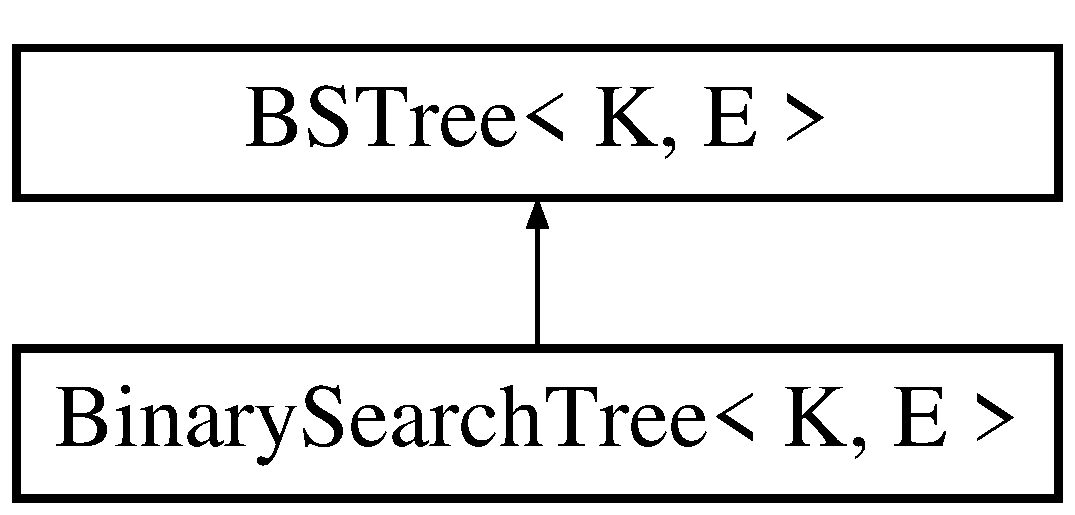
\includegraphics[height=2.000000cm]{classBSTree}
\end{center}
\end{figure}
\subsection*{Public Member Functions}
\begin{DoxyCompactItemize}
\item 
\mbox{\Hypertarget{classBSTree_aef2c4b7362084b3aa5c10175f0d120ca}\label{classBSTree_aef2c4b7362084b3aa5c10175f0d120ca}} 
virtual const pair$<$ const K, E $>$ {\bfseries find} (const K \&) const =0
\item 
\mbox{\Hypertarget{classBSTree_aa504fb22644d5f492adeb0a75c5c34ad}\label{classBSTree_aa504fb22644d5f492adeb0a75c5c34ad}} 
virtual void {\bfseries insert} (const pair$<$ const K, E $>$ \&)=0
\item 
\mbox{\Hypertarget{classBSTree_a875bb53c8b086d7d61d9b65eb89ed6d1}\label{classBSTree_a875bb53c8b086d7d61d9b65eb89ed6d1}} 
virtual void {\bfseries erase} (const K \&)=0
\item 
\mbox{\Hypertarget{classBSTree_a04ddff6640edd09c9b394d409157c225}\label{classBSTree_a04ddff6640edd09c9b394d409157c225}} 
virtual void {\bfseries ascend} ()=0
\end{DoxyCompactItemize}


The documentation for this class was generated from the following file\+:\begin{DoxyCompactItemize}
\item 
data\+\_\+structure/tree/binary\+\_\+search\+\_\+tree.\+h\end{DoxyCompactItemize}

\hypertarget{classClient}{}\section{Client Class Reference}
\label{classClient}\index{Client@{Client}}
\subsection*{Public Types}
\begin{DoxyCompactItemize}
\item 
\mbox{\Hypertarget{classClient_a03f58c98b8df3579787a6eccc298ab4a}\label{classClient_a03f58c98b8df3579787a6eccc298ab4a}} 
typedef std\+::shared\+\_\+ptr$<$ ip\+::tcp\+::socket $>$ {\bfseries socket\+\_\+ptr}
\end{DoxyCompactItemize}
\subsection*{Public Member Functions}
\begin{DoxyCompactItemize}
\item 
\mbox{\Hypertarget{classClient_a2b0ae820b15a019267b423d0363ea101}\label{classClient_a2b0ae820b15a019267b423d0363ea101}} 
{\bfseries Client} (io\+\_\+service \&ser)
\item 
\mbox{\Hypertarget{classClient_a742373e08a80d993d2651b6fff76f5b9}\label{classClient_a742373e08a80d993d2651b6fff76f5b9}} 
void {\bfseries start} ()
\end{DoxyCompactItemize}
\subsection*{Private Member Functions}
\begin{DoxyCompactItemize}
\item 
\mbox{\Hypertarget{classClient_a5011794316f35956bd84e936d6901a56}\label{classClient_a5011794316f35956bd84e936d6901a56}} 
void {\bfseries start\+\_\+connect} (socket\+\_\+ptr psocket)
\item 
\mbox{\Hypertarget{classClient_a597b228a77ab86e302ec96334c797843}\label{classClient_a597b228a77ab86e302ec96334c797843}} 
void {\bfseries handle\+\_\+connect} (socket\+\_\+ptr psocket, const boost\+::system\+::error\+\_\+code ec)
\end{DoxyCompactItemize}
\subsection*{Private Attributes}
\begin{DoxyCompactItemize}
\item 
\mbox{\Hypertarget{classClient_ac0a4b8c27ad244474468d01ac3196251}\label{classClient_ac0a4b8c27ad244474468d01ac3196251}} 
io\+\_\+service \& {\bfseries service}
\item 
\mbox{\Hypertarget{classClient_ac9ba36c4dc3810ff4cab07a250b9b78d}\label{classClient_ac9ba36c4dc3810ff4cab07a250b9b78d}} 
ip\+::tcp\+::endpoint {\bfseries ep}
\end{DoxyCompactItemize}


The documentation for this class was generated from the following file\+:\begin{DoxyCompactItemize}
\item 
asio/async\+\_\+client.\+cc\end{DoxyCompactItemize}

\hypertarget{classcmp}{}\section{cmp$<$ T $>$ Class Template Reference}
\label{classcmp}\index{cmp$<$ T $>$@{cmp$<$ T $>$}}
\subsection*{Public Member Functions}
\begin{DoxyCompactItemize}
\item 
\mbox{\Hypertarget{classcmp_a63c82fa7008ab4338fab59cd7cae753a}\label{classcmp_a63c82fa7008ab4338fab59cd7cae753a}} 
bool {\bfseries operator()} (const \hyperlink{structHuffmanNode}{Huffman\+Node}$<$ T $>$ n, const \hyperlink{structHuffmanNode}{Huffman\+Node}$<$ T $>$ m)
\end{DoxyCompactItemize}


The documentation for this class was generated from the following file\+:\begin{DoxyCompactItemize}
\item 
data\+\_\+structure/tree/huffman\+\_\+tree.\+cc\end{DoxyCompactItemize}

\hypertarget{classCompleteWinnerTree}{}\section{Complete\+Winner\+Tree$<$ T $>$ Class Template Reference}
\label{classCompleteWinnerTree}\index{Complete\+Winner\+Tree$<$ T $>$@{Complete\+Winner\+Tree$<$ T $>$}}
Inheritance diagram for Complete\+Winner\+Tree$<$ T $>$\+:\begin{figure}[H]
\begin{center}
\leavevmode
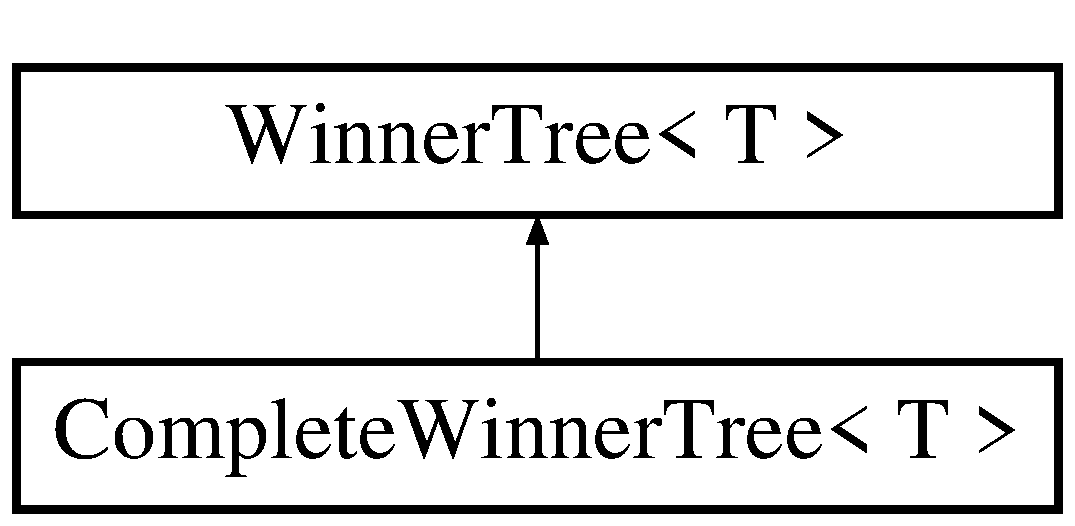
\includegraphics[height=2.000000cm]{classCompleteWinnerTree}
\end{center}
\end{figure}
\subsection*{Public Member Functions}
\begin{DoxyCompactItemize}
\item 
\mbox{\Hypertarget{classCompleteWinnerTree_aa2634870d578aacdeeb9a7ae5ce9d078}\label{classCompleteWinnerTree_aa2634870d578aacdeeb9a7ae5ce9d078}} 
{\bfseries Complete\+Winner\+Tree} (T $\ast$array, int num)
\item 
\mbox{\Hypertarget{classCompleteWinnerTree_a9c7cf644a3051d4ed3e02fb5da53dcf1}\label{classCompleteWinnerTree_a9c7cf644a3051d4ed3e02fb5da53dcf1}} 
void {\bfseries initialize} (T $\ast$, int)
\item 
\mbox{\Hypertarget{classCompleteWinnerTree_abc4419384c68a0b08b8fa3fbfb1d6238}\label{classCompleteWinnerTree_abc4419384c68a0b08b8fa3fbfb1d6238}} 
size\+\_\+t {\bfseries winner} ()
\item 
\mbox{\Hypertarget{classCompleteWinnerTree_a0e9092b85b87a0083746bea27368c587}\label{classCompleteWinnerTree_a0e9092b85b87a0083746bea27368c587}} 
void {\bfseries replay} (size\+\_\+t)
\end{DoxyCompactItemize}
\subsection*{Private Member Functions}
\begin{DoxyCompactItemize}
\item 
\mbox{\Hypertarget{classCompleteWinnerTree_a284633037345aff8d7f87400b2ebc0eb}\label{classCompleteWinnerTree_a284633037345aff8d7f87400b2ebc0eb}} 
size\+\_\+t {\bfseries max} (size\+\_\+t n, size\+\_\+t m)
\end{DoxyCompactItemize}
\subsection*{Private Attributes}
\begin{DoxyCompactItemize}
\item 
\mbox{\Hypertarget{classCompleteWinnerTree_adc3e56f07e19d3e82bcc838e7ff19ee6}\label{classCompleteWinnerTree_adc3e56f07e19d3e82bcc838e7ff19ee6}} 
T $\ast$ {\bfseries player}
\item 
\mbox{\Hypertarget{classCompleteWinnerTree_a2d98d5cf839969d302e234b3476b6657}\label{classCompleteWinnerTree_a2d98d5cf839969d302e234b3476b6657}} 
size\+\_\+t $\ast$ {\bfseries tree}
\item 
\mbox{\Hypertarget{classCompleteWinnerTree_a2f955e8e6a28e10047ab0c0bc9130d5d}\label{classCompleteWinnerTree_a2f955e8e6a28e10047ab0c0bc9130d5d}} 
size\+\_\+t {\bfseries player\+\_\+num}
\end{DoxyCompactItemize}


The documentation for this class was generated from the following file\+:\begin{DoxyCompactItemize}
\item 
data\+\_\+structure/tree/winner\+\_\+tree.\+h\end{DoxyCompactItemize}

\hypertarget{classCRedisPublisher}{}\section{C\+Redis\+Publisher Class Reference}
\label{classCRedisPublisher}\index{C\+Redis\+Publisher@{C\+Redis\+Publisher}}
\subsection*{Public Member Functions}
\begin{DoxyCompactItemize}
\item 
\mbox{\Hypertarget{classCRedisPublisher_ac133099f447b301fa406f43e53d2fcb7}\label{classCRedisPublisher_ac133099f447b301fa406f43e53d2fcb7}} 
bool {\bfseries init} ()
\item 
\mbox{\Hypertarget{classCRedisPublisher_a023c98d3b0d2bbd6bd0e9d6c038f4fcf}\label{classCRedisPublisher_a023c98d3b0d2bbd6bd0e9d6c038f4fcf}} 
bool {\bfseries uninit} ()
\item 
\mbox{\Hypertarget{classCRedisPublisher_ae042c9b8e0aa35d831f407add0d5a09d}\label{classCRedisPublisher_ae042c9b8e0aa35d831f407add0d5a09d}} 
bool {\bfseries connect} ()
\item 
\mbox{\Hypertarget{classCRedisPublisher_aa359b52013c6120445631fa89902613d}\label{classCRedisPublisher_aa359b52013c6120445631fa89902613d}} 
bool {\bfseries disconnect} ()
\item 
\mbox{\Hypertarget{classCRedisPublisher_a4e8b402ae6b39806424c37e74598b242}\label{classCRedisPublisher_a4e8b402ae6b39806424c37e74598b242}} 
bool {\bfseries publish} (const std\+::string \&channel\+\_\+name, const std\+::string \&message)
\end{DoxyCompactItemize}
\subsection*{Private Member Functions}
\begin{DoxyCompactItemize}
\item 
\mbox{\Hypertarget{classCRedisPublisher_ac9333f0b59f7779fb803fc12020680df}\label{classCRedisPublisher_ac9333f0b59f7779fb803fc12020680df}} 
void $\ast$ {\bfseries event\+\_\+proc} ()
\end{DoxyCompactItemize}
\subsection*{Static Private Member Functions}
\begin{DoxyCompactItemize}
\item 
\mbox{\Hypertarget{classCRedisPublisher_a12d4cfd9ca003dfdcc47695f7f840092}\label{classCRedisPublisher_a12d4cfd9ca003dfdcc47695f7f840092}} 
static void {\bfseries connect\+\_\+callback} (const redis\+Async\+Context $\ast$redis\+\_\+context, int status)
\item 
\mbox{\Hypertarget{classCRedisPublisher_ac801e3e460d44b75452831901fcae604}\label{classCRedisPublisher_ac801e3e460d44b75452831901fcae604}} 
static void {\bfseries disconnect\+\_\+callback} (const redis\+Async\+Context $\ast$redis\+\_\+context, int status)
\item 
\mbox{\Hypertarget{classCRedisPublisher_ac223c0ccd3e246f513341680edda6c46}\label{classCRedisPublisher_ac223c0ccd3e246f513341680edda6c46}} 
static void {\bfseries command\+\_\+callback} (redis\+Async\+Context $\ast$redis\+\_\+context, void $\ast$reply, void $\ast$privdata)
\item 
\mbox{\Hypertarget{classCRedisPublisher_abdc8924997c801b5f0aad2107c95ca6f}\label{classCRedisPublisher_abdc8924997c801b5f0aad2107c95ca6f}} 
static void $\ast$ {\bfseries event\+\_\+thread} (void $\ast$data)
\end{DoxyCompactItemize}
\subsection*{Private Attributes}
\begin{DoxyCompactItemize}
\item 
\mbox{\Hypertarget{classCRedisPublisher_ab34e87bdea5ef0c98f676077bf3c2e3f}\label{classCRedisPublisher_ab34e87bdea5ef0c98f676077bf3c2e3f}} 
event\+\_\+base $\ast$ {\bfseries \+\_\+event\+\_\+base}
\item 
\mbox{\Hypertarget{classCRedisPublisher_a9e2d7f6e5baa11065b9a88ad0139ed18}\label{classCRedisPublisher_a9e2d7f6e5baa11065b9a88ad0139ed18}} 
pthread\+\_\+t {\bfseries \+\_\+event\+\_\+thread}
\item 
\mbox{\Hypertarget{classCRedisPublisher_aac6ab16975e7015913ccb236c7e707ed}\label{classCRedisPublisher_aac6ab16975e7015913ccb236c7e707ed}} 
sem\+\_\+t {\bfseries \+\_\+event\+\_\+sem}
\item 
\mbox{\Hypertarget{classCRedisPublisher_a02c6968c1e60451e0278e4c1df2f8da0}\label{classCRedisPublisher_a02c6968c1e60451e0278e4c1df2f8da0}} 
redis\+Async\+Context $\ast$ {\bfseries \+\_\+redis\+\_\+context}
\end{DoxyCompactItemize}


The documentation for this class was generated from the following files\+:\begin{DoxyCompactItemize}
\item 
redis/subscriber/redis\+\_\+publisher.\+h\item 
redis/subscriber/redis\+\_\+publisher.\+cc\end{DoxyCompactItemize}

\hypertarget{classCRedisSubscriber}{}\section{C\+Redis\+Subscriber Class Reference}
\label{classCRedisSubscriber}\index{C\+Redis\+Subscriber@{C\+Redis\+Subscriber}}
\subsection*{Public Types}
\begin{DoxyCompactItemize}
\item 
\mbox{\Hypertarget{classCRedisSubscriber_aed46e92256f595ea9e6198b64aa3be84}\label{classCRedisSubscriber_aed46e92256f595ea9e6198b64aa3be84}} 
typedef std\+::tr1\+::function$<$ void(const char $\ast$, const char $\ast$, int)$>$ {\bfseries Notify\+Message\+Fn}
\end{DoxyCompactItemize}
\subsection*{Public Member Functions}
\begin{DoxyCompactItemize}
\item 
\mbox{\Hypertarget{classCRedisSubscriber_afef590bbd6fde34b17089d401ef4dac5}\label{classCRedisSubscriber_afef590bbd6fde34b17089d401ef4dac5}} 
bool {\bfseries init} (const Notify\+Message\+Fn \&fn)
\item 
\mbox{\Hypertarget{classCRedisSubscriber_a12ff40e571587e147e5049ca25e0d2bc}\label{classCRedisSubscriber_a12ff40e571587e147e5049ca25e0d2bc}} 
bool {\bfseries uninit} ()
\item 
\mbox{\Hypertarget{classCRedisSubscriber_a4a5cfff21256fd1b87410f91f5a41595}\label{classCRedisSubscriber_a4a5cfff21256fd1b87410f91f5a41595}} 
bool {\bfseries connect} ()
\item 
\mbox{\Hypertarget{classCRedisSubscriber_ad6a929b69868697ec06d5eb97d58c84c}\label{classCRedisSubscriber_ad6a929b69868697ec06d5eb97d58c84c}} 
bool {\bfseries disconnect} ()
\item 
\mbox{\Hypertarget{classCRedisSubscriber_a6f39a0e6070a25263a72373ee84ac1ba}\label{classCRedisSubscriber_a6f39a0e6070a25263a72373ee84ac1ba}} 
bool {\bfseries subscribe} (const std\+::string \&channel\+\_\+name)
\end{DoxyCompactItemize}
\subsection*{Private Member Functions}
\begin{DoxyCompactItemize}
\item 
\mbox{\Hypertarget{classCRedisSubscriber_a348b74323ec1771429631b7bbf4226c6}\label{classCRedisSubscriber_a348b74323ec1771429631b7bbf4226c6}} 
void $\ast$ {\bfseries event\+\_\+proc} ()
\end{DoxyCompactItemize}
\subsection*{Static Private Member Functions}
\begin{DoxyCompactItemize}
\item 
\mbox{\Hypertarget{classCRedisSubscriber_aa77a510f25ffb7376ba6b183a6b48067}\label{classCRedisSubscriber_aa77a510f25ffb7376ba6b183a6b48067}} 
static void {\bfseries connect\+\_\+callback} (const redis\+Async\+Context $\ast$redis\+\_\+context, int status)
\item 
\mbox{\Hypertarget{classCRedisSubscriber_a05bfb1d0a0970d1eaa24b9bc68ed926b}\label{classCRedisSubscriber_a05bfb1d0a0970d1eaa24b9bc68ed926b}} 
static void {\bfseries disconnect\+\_\+callback} (const redis\+Async\+Context $\ast$redis\+\_\+context, int status)
\item 
\mbox{\Hypertarget{classCRedisSubscriber_a1e7f2f8bc19c02959029d8f07de369f7}\label{classCRedisSubscriber_a1e7f2f8bc19c02959029d8f07de369f7}} 
static void {\bfseries command\+\_\+callback} (redis\+Async\+Context $\ast$redis\+\_\+context, void $\ast$reply, void $\ast$privdata)
\item 
\mbox{\Hypertarget{classCRedisSubscriber_acaf0189862d3b1e670bbb7faed00a9b5}\label{classCRedisSubscriber_acaf0189862d3b1e670bbb7faed00a9b5}} 
static void $\ast$ {\bfseries event\+\_\+thread} (void $\ast$data)
\end{DoxyCompactItemize}
\subsection*{Private Attributes}
\begin{DoxyCompactItemize}
\item 
\mbox{\Hypertarget{classCRedisSubscriber_ac8315d268596c9428b680a807ec2e201}\label{classCRedisSubscriber_ac8315d268596c9428b680a807ec2e201}} 
event\+\_\+base $\ast$ {\bfseries \+\_\+event\+\_\+base}
\item 
\mbox{\Hypertarget{classCRedisSubscriber_a7000af1ba0864def342aa7b7fd3883be}\label{classCRedisSubscriber_a7000af1ba0864def342aa7b7fd3883be}} 
pthread\+\_\+t {\bfseries \+\_\+event\+\_\+thread}
\item 
\mbox{\Hypertarget{classCRedisSubscriber_adcf026425dfecb08bad1ca652aad0306}\label{classCRedisSubscriber_adcf026425dfecb08bad1ca652aad0306}} 
sem\+\_\+t {\bfseries \+\_\+event\+\_\+sem}
\item 
\mbox{\Hypertarget{classCRedisSubscriber_a10d8a2562050b5906d0e67c83b013aa8}\label{classCRedisSubscriber_a10d8a2562050b5906d0e67c83b013aa8}} 
redis\+Async\+Context $\ast$ {\bfseries \+\_\+redis\+\_\+context}
\item 
\mbox{\Hypertarget{classCRedisSubscriber_abe11c1bbe2c935ac9b59284d2eed708d}\label{classCRedisSubscriber_abe11c1bbe2c935ac9b59284d2eed708d}} 
Notify\+Message\+Fn {\bfseries \+\_\+notify\+\_\+message\+\_\+fn}
\end{DoxyCompactItemize}


The documentation for this class was generated from the following files\+:\begin{DoxyCompactItemize}
\item 
redis/subscriber/redis\+\_\+subscriber.\+h\item 
redis/subscriber/redis\+\_\+subscriber.\+cc\end{DoxyCompactItemize}

\hypertarget{structfunc}{}\section{func Struct Reference}
\label{structfunc}\index{func@{func}}
\subsection*{Public Member Functions}
\begin{DoxyCompactItemize}
\item 
\mbox{\Hypertarget{structfunc_a6801d59dec3f95f3f7e2d9505212f144}\label{structfunc_a6801d59dec3f95f3f7e2d9505212f144}} 
{\bfseries func} (int \&i\+\_\+)
\item 
\mbox{\Hypertarget{structfunc_ae6878437e9e8405fe4f96dd798ef835d}\label{structfunc_ae6878437e9e8405fe4f96dd798ef835d}} 
void {\bfseries operator()} ()
\end{DoxyCompactItemize}
\subsection*{Public Attributes}
\begin{DoxyCompactItemize}
\item 
\mbox{\Hypertarget{structfunc_afe95e62710d2ce5ca8fa9de4fd912a9d}\label{structfunc_afe95e62710d2ce5ca8fa9de4fd912a9d}} 
int \& {\bfseries i}
\item 
\mbox{\Hypertarget{structfunc_a4861931814274b32bc1267cd4999a578}\label{structfunc_a4861931814274b32bc1267cd4999a578}} 
int {\bfseries n}
\end{DoxyCompactItemize}


The documentation for this struct was generated from the following file\+:\begin{DoxyCompactItemize}
\item 
thread/test\+\_\+temp.\+cc\end{DoxyCompactItemize}

\hypertarget{classgraph}{}\section{graph$<$ T $>$ Class Template Reference}
\label{classgraph}\index{graph$<$ T $>$@{graph$<$ T $>$}}
Inheritance diagram for graph$<$ T $>$\+:\begin{figure}[H]
\begin{center}
\leavevmode
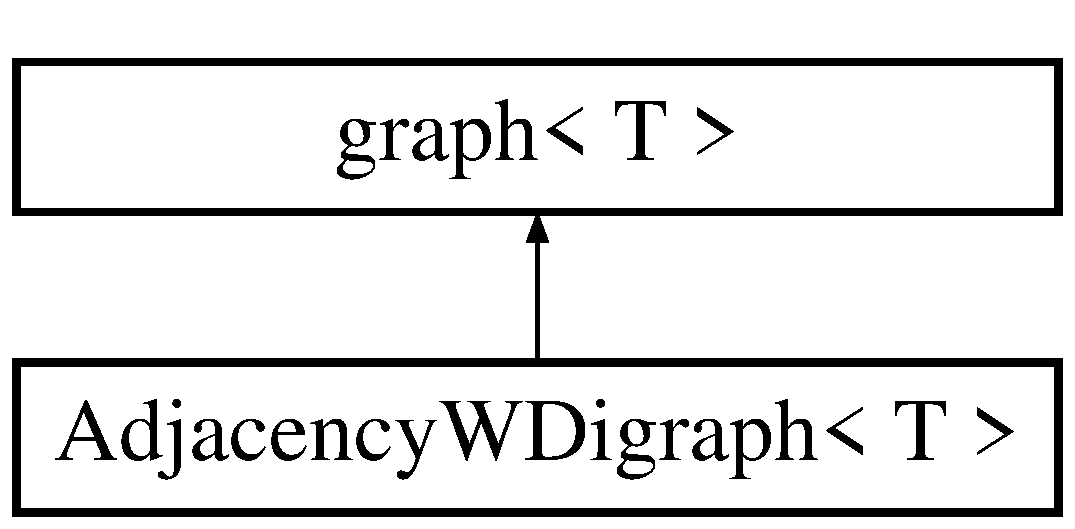
\includegraphics[height=2.000000cm]{classgraph}
\end{center}
\end{figure}
\subsection*{Public Member Functions}
\begin{DoxyCompactItemize}
\item 
\mbox{\Hypertarget{classgraph_a09d38d3a6517294b919153d8040e6ec3}\label{classgraph_a09d38d3a6517294b919153d8040e6ec3}} 
virtual int {\bfseries num\+\_\+of\+\_\+vertices} () const =0
\item 
\mbox{\Hypertarget{classgraph_a3c5db2574a9a7ddfd44e8f2f5c4d713e}\label{classgraph_a3c5db2574a9a7ddfd44e8f2f5c4d713e}} 
virtual int {\bfseries num\+\_\+of\+\_\+edges} () const =0
\item 
\mbox{\Hypertarget{classgraph_a252a14b0bf9b10bcfdfec83df07c60b5}\label{classgraph_a252a14b0bf9b10bcfdfec83df07c60b5}} 
virtual bool {\bfseries exists\+\_\+edge} (int, int) const =0
\item 
\mbox{\Hypertarget{classgraph_aa9e0efd15c95887ec7d9a82bf36e1704}\label{classgraph_aa9e0efd15c95887ec7d9a82bf36e1704}} 
virtual void {\bfseries insert\+\_\+edge} (int, int, T)=0
\item 
\mbox{\Hypertarget{classgraph_ad0d12d6f8e6e2881e7d5f5ed732acc8a}\label{classgraph_ad0d12d6f8e6e2881e7d5f5ed732acc8a}} 
virtual void {\bfseries erase\+\_\+edge} (int, int)=0
\item 
\mbox{\Hypertarget{classgraph_a3ac37382a706f5ad8a76a4f3439843b3}\label{classgraph_a3ac37382a706f5ad8a76a4f3439843b3}} 
virtual int {\bfseries degree} (int) const =0
\item 
\mbox{\Hypertarget{classgraph_a9f37d81c0bbbd854e55e5a83f98871d4}\label{classgraph_a9f37d81c0bbbd854e55e5a83f98871d4}} 
virtual int {\bfseries in\+\_\+degree} (int) const =0
\item 
\mbox{\Hypertarget{classgraph_aceb953196b3fc06e3eda715311c70542}\label{classgraph_aceb953196b3fc06e3eda715311c70542}} 
virtual int {\bfseries out\+\_\+degree} (int) const =0
\item 
\mbox{\Hypertarget{classgraph_a583ec6a74dd86daea97410ebeb7e7989}\label{classgraph_a583ec6a74dd86daea97410ebeb7e7989}} 
virtual bool {\bfseries directed} () const =0
\item 
\mbox{\Hypertarget{classgraph_ab84679f42eca64f8395b331ed27cdf14}\label{classgraph_ab84679f42eca64f8395b331ed27cdf14}} 
virtual bool {\bfseries weighted} () const =0
\item 
\mbox{\Hypertarget{classgraph_a187b0c9dac2d5b3d7d2c21b4f80047c8}\label{classgraph_a187b0c9dac2d5b3d7d2c21b4f80047c8}} 
virtual \hyperlink{classvertex__iterator}{vertex\+\_\+iterator}$<$ T $>$ $\ast$ {\bfseries iterator} (int)=0
\item 
\mbox{\Hypertarget{classgraph_a2b8224ad27463b099c4b21b090a8a468}\label{classgraph_a2b8224ad27463b099c4b21b090a8a468}} 
virtual void {\bfseries bfs} (int, int\mbox{[}$\,$\mbox{]}, int)
\item 
\mbox{\Hypertarget{classgraph_a7c2a8cef100e1f3721405ec3a0c143d5}\label{classgraph_a7c2a8cef100e1f3721405ec3a0c143d5}} 
virtual void {\bfseries dfs} (int, int\mbox{[}$\,$\mbox{]}, int)
\end{DoxyCompactItemize}


The documentation for this class was generated from the following file\+:\begin{DoxyCompactItemize}
\item 
data\+\_\+structure/graph/graph.\+h\end{DoxyCompactItemize}

\hypertarget{structHuffmanNode}{}\section{Huffman\+Node$<$ T $>$ Struct Template Reference}
\label{structHuffmanNode}\index{Huffman\+Node$<$ T $>$@{Huffman\+Node$<$ T $>$}}
\subsection*{Public Member Functions}
\begin{DoxyCompactItemize}
\item 
\mbox{\Hypertarget{structHuffmanNode_a5aba43634df75a97b2114baba4dfb123}\label{structHuffmanNode_a5aba43634df75a97b2114baba4dfb123}} 
{\bfseries Huffman\+Node} (\hyperlink{classLinkedBinaryTree}{Linked\+Binary\+Tree}$<$ size\+\_\+t $>$ $\ast$ptree, T weight)
\end{DoxyCompactItemize}
\subsection*{Public Attributes}
\begin{DoxyCompactItemize}
\item 
\mbox{\Hypertarget{structHuffmanNode_ad4779f77355c50735e51fde718f7dc1e}\label{structHuffmanNode_ad4779f77355c50735e51fde718f7dc1e}} 
\hyperlink{classLinkedBinaryTree}{Linked\+Binary\+Tree}$<$ size\+\_\+t $>$ $\ast$ {\bfseries tree}
\item 
\mbox{\Hypertarget{structHuffmanNode_a213b1555f15afc248eb7ec5843f6280a}\label{structHuffmanNode_a213b1555f15afc248eb7ec5843f6280a}} 
T {\bfseries weight}
\end{DoxyCompactItemize}


The documentation for this struct was generated from the following file\+:\begin{DoxyCompactItemize}
\item 
data\+\_\+structure/tree/huffman\+\_\+tree.\+cc\end{DoxyCompactItemize}

\hypertarget{classiterator}{}\section{iterator$<$ T $>$ Class Template Reference}
\label{classiterator}\index{iterator$<$ T $>$@{iterator$<$ T $>$}}
\subsection*{Public Types}
\begin{DoxyCompactItemize}
\item 
\mbox{\Hypertarget{classiterator_a743a266afa7b73c484bf74461c100eb9}\label{classiterator_a743a266afa7b73c484bf74461c100eb9}} 
typedef std\+::bidirectional\+\_\+iterator\+\_\+tag {\bfseries iterator\+\_\+category}
\item 
\mbox{\Hypertarget{classiterator_a3000f949e77f12b9d25292e47e6c9d94}\label{classiterator_a3000f949e77f12b9d25292e47e6c9d94}} 
typedef T {\bfseries value\+\_\+type}
\item 
\mbox{\Hypertarget{classiterator_a9bfdd911ffa5ac8414b56118ecb6722e}\label{classiterator_a9bfdd911ffa5ac8414b56118ecb6722e}} 
typedef std\+::ptrdiff\+\_\+t {\bfseries difference\+\_\+type}
\item 
\mbox{\Hypertarget{classiterator_aff916de6b5d0d925c095ff69e50dcc2e}\label{classiterator_aff916de6b5d0d925c095ff69e50dcc2e}} 
typedef T $\ast$ {\bfseries pointer}
\item 
\mbox{\Hypertarget{classiterator_ab4cb4c59c8799e17f6a2e6a59b9c31f1}\label{classiterator_ab4cb4c59c8799e17f6a2e6a59b9c31f1}} 
typedef T \& {\bfseries referrnce}
\end{DoxyCompactItemize}
\subsection*{Public Member Functions}
\begin{DoxyCompactItemize}
\item 
\mbox{\Hypertarget{classiterator_aeefbadab3a70434fd7209e53cfde1eda}\label{classiterator_aeefbadab3a70434fd7209e53cfde1eda}} 
{\bfseries iterator} (T $\ast$the\+Position)
\item 
\mbox{\Hypertarget{classiterator_a812b6eb54f898651c5f3843d3bc6b304}\label{classiterator_a812b6eb54f898651c5f3843d3bc6b304}} 
T \& {\bfseries operator$\ast$} () const
\item 
\mbox{\Hypertarget{classiterator_ac6dc72b0fe61dd7eaff65dae06f546e6}\label{classiterator_ac6dc72b0fe61dd7eaff65dae06f546e6}} 
T \& {\bfseries operator-\/$>$} () const
\item 
\mbox{\Hypertarget{classiterator_ac7aa9929d22f3537fec4199f78d5ea0f}\label{classiterator_ac7aa9929d22f3537fec4199f78d5ea0f}} 
\hyperlink{classiterator}{iterator} \& {\bfseries operator++} ()
\item 
\mbox{\Hypertarget{classiterator_aee23ee83b4ada171ef7b5d84023a9a86}\label{classiterator_aee23ee83b4ada171ef7b5d84023a9a86}} 
\hyperlink{classiterator}{iterator} {\bfseries operator++} (int)
\item 
\mbox{\Hypertarget{classiterator_aece894a066138fd746018c25b66aa21b}\label{classiterator_aece894a066138fd746018c25b66aa21b}} 
\hyperlink{classiterator}{iterator} \& {\bfseries operator-\/-\/} ()
\item 
\mbox{\Hypertarget{classiterator_a03399efe64e2576f58af280a93f6b0e2}\label{classiterator_a03399efe64e2576f58af280a93f6b0e2}} 
\hyperlink{classiterator}{iterator} {\bfseries operator-\/-\/} (int)
\item 
\mbox{\Hypertarget{classiterator_a41525a41e1b5975155f4908c3446163f}\label{classiterator_a41525a41e1b5975155f4908c3446163f}} 
bool {\bfseries operator!=} (const \hyperlink{classiterator}{iterator} \&rhs) const
\item 
\mbox{\Hypertarget{classiterator_af5ae5f2473c7b117149354b660ce7cfd}\label{classiterator_af5ae5f2473c7b117149354b660ce7cfd}} 
bool {\bfseries operator==} (const \hyperlink{classiterator}{iterator} \&rhs) const
\end{DoxyCompactItemize}
\subsection*{Protected Attributes}
\begin{DoxyCompactItemize}
\item 
\mbox{\Hypertarget{classiterator_ad4b129783502be6635bb37f463ba0998}\label{classiterator_ad4b129783502be6635bb37f463ba0998}} 
T $\ast$ {\bfseries position}
\end{DoxyCompactItemize}


The documentation for this class was generated from the following file\+:\begin{DoxyCompactItemize}
\item 
data\+\_\+structure/linear\+\_\+list/array\+\_\+list.\+h\end{DoxyCompactItemize}

\hypertarget{classLinearList}{}\section{Linear\+List$<$ T $>$ Class Template Reference}
\label{classLinearList}\index{Linear\+List$<$ T $>$@{Linear\+List$<$ T $>$}}
Inheritance diagram for Linear\+List$<$ T $>$\+:\begin{figure}[H]
\begin{center}
\leavevmode
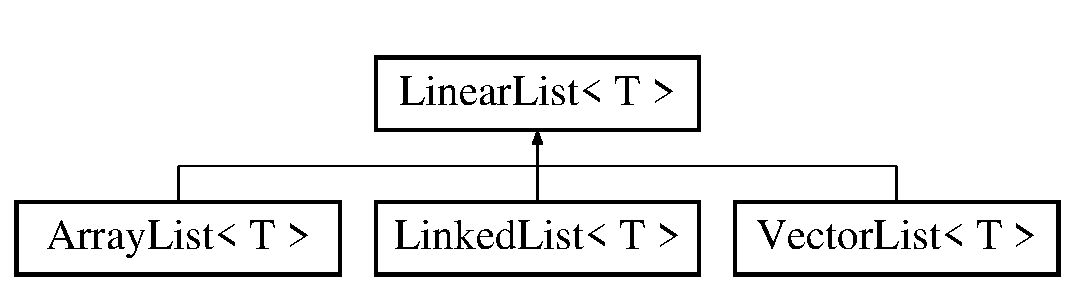
\includegraphics[height=2.000000cm]{classLinearList}
\end{center}
\end{figure}
\subsection*{Public Member Functions}
\begin{DoxyCompactItemize}
\item 
\mbox{\Hypertarget{classLinearList_ad7ddf5d1f6625f9c2c92f2fa12e46dbd}\label{classLinearList_ad7ddf5d1f6625f9c2c92f2fa12e46dbd}} 
virtual bool {\bfseries empty} () const =0
\item 
\mbox{\Hypertarget{classLinearList_a8db72437c90cd51fca0a72ad737a58e8}\label{classLinearList_a8db72437c90cd51fca0a72ad737a58e8}} 
virtual int {\bfseries size} () const =0
\item 
\mbox{\Hypertarget{classLinearList_add1333f53468ffeb7274e660cf524f64}\label{classLinearList_add1333f53468ffeb7274e660cf524f64}} 
virtual T \& {\bfseries get} (int the\+Index) const =0
\item 
\mbox{\Hypertarget{classLinearList_a73f1f5c7bb9cee830393bb29c7b4b934}\label{classLinearList_a73f1f5c7bb9cee830393bb29c7b4b934}} 
virtual int {\bfseries index\+Of} (const T \&the\+Element) const =0
\item 
\mbox{\Hypertarget{classLinearList_a11b88599d63152661e6a8c17b518102e}\label{classLinearList_a11b88599d63152661e6a8c17b518102e}} 
virtual void {\bfseries erase} (int the\+Index)=0
\item 
\mbox{\Hypertarget{classLinearList_a5fbe118bc2462a56f882bfaf9572627a}\label{classLinearList_a5fbe118bc2462a56f882bfaf9572627a}} 
virtual void {\bfseries insert} (int the\+Index, const T \&the\+Element)=0
\item 
\mbox{\Hypertarget{classLinearList_a33a29cad0a20f500dd8da6dc64a7b565}\label{classLinearList_a33a29cad0a20f500dd8da6dc64a7b565}} 
virtual void {\bfseries output} (std\+::ostream \&out) const =0
\end{DoxyCompactItemize}


The documentation for this class was generated from the following file\+:\begin{DoxyCompactItemize}
\item 
data\+\_\+structure/linear\+\_\+list/linear\+\_\+list.\+h\end{DoxyCompactItemize}

\hypertarget{classLinkedBinaryTree}{}\section{Linked\+Binary\+Tree$<$ T $>$ Class Template Reference}
\label{classLinkedBinaryTree}\index{Linked\+Binary\+Tree$<$ T $>$@{Linked\+Binary\+Tree$<$ T $>$}}
Inheritance diagram for Linked\+Binary\+Tree$<$ T $>$\+:\begin{figure}[H]
\begin{center}
\leavevmode
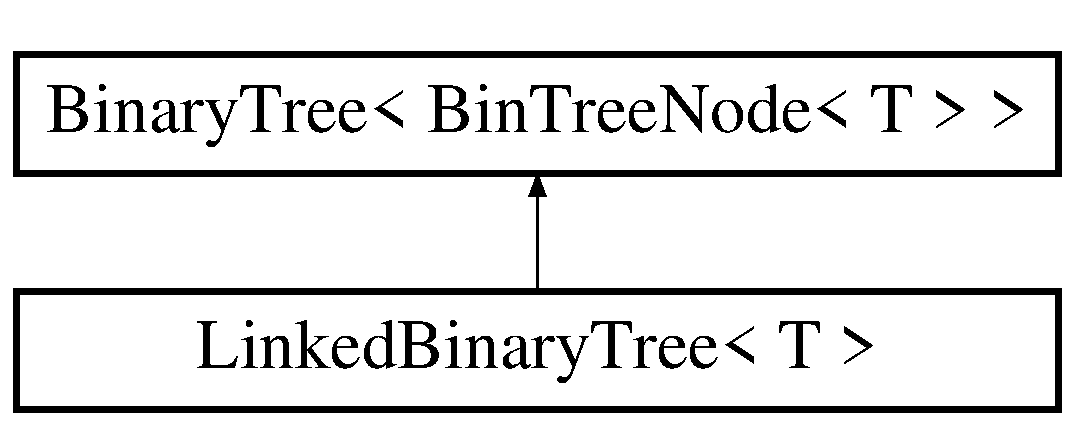
\includegraphics[height=2.000000cm]{classLinkedBinaryTree}
\end{center}
\end{figure}
\subsection*{Public Member Functions}
\begin{DoxyCompactItemize}
\item 
\mbox{\Hypertarget{classLinkedBinaryTree_af79026e3ff32394af7fa4bc17104b2f2}\label{classLinkedBinaryTree_af79026e3ff32394af7fa4bc17104b2f2}} 
{\bfseries Linked\+Binary\+Tree} (const \hyperlink{classLinkedBinaryTree}{Linked\+Binary\+Tree}$<$ T $>$ \&tree)
\item 
\mbox{\Hypertarget{classLinkedBinaryTree_a1c77aca3aaa8ff25dbacf718b6277fbf}\label{classLinkedBinaryTree_a1c77aca3aaa8ff25dbacf718b6277fbf}} 
{\bfseries Linked\+Binary\+Tree} (T element, \hyperlink{classLinkedBinaryTree}{Linked\+Binary\+Tree}$<$ T $>$ $\ast$left, \hyperlink{classLinkedBinaryTree}{Linked\+Binary\+Tree}$<$ T $>$ $\ast$right)
\item 
\mbox{\Hypertarget{classLinkedBinaryTree_a31090e85a7b2a6b8cad23717ec433ceb}\label{classLinkedBinaryTree_a31090e85a7b2a6b8cad23717ec433ceb}} 
bool {\bfseries empty} () const
\item 
\mbox{\Hypertarget{classLinkedBinaryTree_a7ec639d841538074a028211d9a4362e8}\label{classLinkedBinaryTree_a7ec639d841538074a028211d9a4362e8}} 
size\+\_\+t {\bfseries size} () const
\item 
\mbox{\Hypertarget{classLinkedBinaryTree_a61115f0284fc3ab3ff46fe24a2ba83e9}\label{classLinkedBinaryTree_a61115f0284fc3ab3ff46fe24a2ba83e9}} 
void {\bfseries Make\+Tree} ()
\item 
void \hyperlink{classLinkedBinaryTree_ab6a897c3961294d56cd83790aaa3ff9c}{Pre\+Order} (void($\ast$visit)(\hyperlink{structBinTreeNode}{Bin\+Tree\+Node}$<$ T $>$ $\ast$))
\item 
void \hyperlink{classLinkedBinaryTree_a82b1a5995e90671905da7502d7f58eba}{In\+Order} (void($\ast$visit)(\hyperlink{structBinTreeNode}{Bin\+Tree\+Node}$<$ T $>$ $\ast$))
\item 
void \hyperlink{classLinkedBinaryTree_ad8a0144cc092a677eb2b3189059dd19f}{Post\+Order} (void($\ast$visit)(\hyperlink{structBinTreeNode}{Bin\+Tree\+Node}$<$ T $>$ $\ast$))
\item 
void \hyperlink{classLinkedBinaryTree_a5ca48cd9b784ca7cdf0f41d03dbc4873}{Level\+Order} (void($\ast$visit)(\hyperlink{structBinTreeNode}{Bin\+Tree\+Node}$<$ T $>$ $\ast$))
\item 
\mbox{\Hypertarget{classLinkedBinaryTree_a43286c1f8b340ff84e73a0f103ebbfe2}\label{classLinkedBinaryTree_a43286c1f8b340ff84e73a0f103ebbfe2}} 
void {\bfseries erase} ()
\item 
\mbox{\Hypertarget{classLinkedBinaryTree_a186b387b4f08ca1abfbcd26b37e56fc3}\label{classLinkedBinaryTree_a186b387b4f08ca1abfbcd26b37e56fc3}} 
void {\bfseries Pre\+Order\+Output} ()
\item 
\mbox{\Hypertarget{classLinkedBinaryTree_ae9d3b8ff0ca1850789023991794b00cf}\label{classLinkedBinaryTree_ae9d3b8ff0ca1850789023991794b00cf}} 
int {\bfseries height} () const
\item 
\mbox{\Hypertarget{classLinkedBinaryTree_af79026e3ff32394af7fa4bc17104b2f2}\label{classLinkedBinaryTree_af79026e3ff32394af7fa4bc17104b2f2}} 
{\bfseries Linked\+Binary\+Tree} (const \hyperlink{classLinkedBinaryTree}{Linked\+Binary\+Tree}$<$ T $>$ \&tree)
\item 
\mbox{\Hypertarget{classLinkedBinaryTree_a31090e85a7b2a6b8cad23717ec433ceb}\label{classLinkedBinaryTree_a31090e85a7b2a6b8cad23717ec433ceb}} 
bool {\bfseries empty} () const
\item 
\mbox{\Hypertarget{classLinkedBinaryTree_a7ec639d841538074a028211d9a4362e8}\label{classLinkedBinaryTree_a7ec639d841538074a028211d9a4362e8}} 
size\+\_\+t {\bfseries size} () const
\item 
\mbox{\Hypertarget{classLinkedBinaryTree_a61115f0284fc3ab3ff46fe24a2ba83e9}\label{classLinkedBinaryTree_a61115f0284fc3ab3ff46fe24a2ba83e9}} 
void {\bfseries Make\+Tree} ()
\item 
\mbox{\Hypertarget{classLinkedBinaryTree_a56d6d694f598016863b7187df9a4f832}\label{classLinkedBinaryTree_a56d6d694f598016863b7187df9a4f832}} 
void {\bfseries Pre\+Order} (void($\ast$visit)(\hyperlink{structRBTreeNode}{R\+B\+Tree\+Node}$<$ T $>$ $\ast$))
\item 
\mbox{\Hypertarget{classLinkedBinaryTree_ab252e8fb5975132a29b85072c79d3786}\label{classLinkedBinaryTree_ab252e8fb5975132a29b85072c79d3786}} 
void {\bfseries In\+Order} (void($\ast$visit)(\hyperlink{structRBTreeNode}{R\+B\+Tree\+Node}$<$ T $>$ $\ast$))
\item 
\mbox{\Hypertarget{classLinkedBinaryTree_a0f89168cebd717b188f8ee25e04bc4e4}\label{classLinkedBinaryTree_a0f89168cebd717b188f8ee25e04bc4e4}} 
void {\bfseries Post\+Order} (void($\ast$visit)(\hyperlink{structRBTreeNode}{R\+B\+Tree\+Node}$<$ T $>$ $\ast$))
\item 
\mbox{\Hypertarget{classLinkedBinaryTree_adf9ff858db2e4a7a44ffdde9009d86dc}\label{classLinkedBinaryTree_adf9ff858db2e4a7a44ffdde9009d86dc}} 
void {\bfseries Level\+Order} (void($\ast$visit)(\hyperlink{structRBTreeNode}{R\+B\+Tree\+Node}$<$ T $>$ $\ast$))
\item 
\mbox{\Hypertarget{classLinkedBinaryTree_a43286c1f8b340ff84e73a0f103ebbfe2}\label{classLinkedBinaryTree_a43286c1f8b340ff84e73a0f103ebbfe2}} 
void {\bfseries erase} ()
\item 
\mbox{\Hypertarget{classLinkedBinaryTree_a186b387b4f08ca1abfbcd26b37e56fc3}\label{classLinkedBinaryTree_a186b387b4f08ca1abfbcd26b37e56fc3}} 
void {\bfseries Pre\+Order\+Output} ()
\item 
\mbox{\Hypertarget{classLinkedBinaryTree_ae9d3b8ff0ca1850789023991794b00cf}\label{classLinkedBinaryTree_ae9d3b8ff0ca1850789023991794b00cf}} 
int {\bfseries height} () const
\end{DoxyCompactItemize}
\subsection*{Static Public Member Functions}
\begin{DoxyCompactItemize}
\item 
\mbox{\Hypertarget{classLinkedBinaryTree_a6ea270a1d0306d6b7b1706dc1b667541}\label{classLinkedBinaryTree_a6ea270a1d0306d6b7b1706dc1b667541}} 
static void {\bfseries Output} (\hyperlink{structBinTreeNode}{Bin\+Tree\+Node}$<$ T $>$ $\ast$t)
\item 
\mbox{\Hypertarget{classLinkedBinaryTree_a3773993f439ae092fcd084decfb6f652}\label{classLinkedBinaryTree_a3773993f439ae092fcd084decfb6f652}} 
static void {\bfseries Output} (\hyperlink{structRBTreeNode}{R\+B\+Tree\+Node}$<$ T $>$ $\ast$t)
\end{DoxyCompactItemize}
\subsection*{Protected Member Functions}
\begin{DoxyCompactItemize}
\item 
\mbox{\Hypertarget{classLinkedBinaryTree_afc338c654fefdada8ea2f83b5eeb59d0}\label{classLinkedBinaryTree_afc338c654fefdada8ea2f83b5eeb59d0}} 
int {\bfseries height} (\hyperlink{structBinTreeNode}{Bin\+Tree\+Node}$<$ T $>$ $\ast$) const
\item 
\mbox{\Hypertarget{classLinkedBinaryTree_a846965fd49048760c3e48e78f456eb47}\label{classLinkedBinaryTree_a846965fd49048760c3e48e78f456eb47}} 
\hyperlink{structBinTreeNode}{Bin\+Tree\+Node}$<$ T $>$ $\ast$ {\bfseries Copy\+Create\+Pre\+Order} (const \hyperlink{structBinTreeNode}{Bin\+Tree\+Node}$<$ T $>$ $\ast$)
\item 
\mbox{\Hypertarget{classLinkedBinaryTree_adeb196927e3e6f99061ed50bedbe4643}\label{classLinkedBinaryTree_adeb196927e3e6f99061ed50bedbe4643}} 
int {\bfseries height} (\hyperlink{structRBTreeNode}{R\+B\+Tree\+Node}$<$ T $>$ $\ast$) const
\item 
\mbox{\Hypertarget{classLinkedBinaryTree_a7e04c9e2d58e7a799be68df531e3e3e1}\label{classLinkedBinaryTree_a7e04c9e2d58e7a799be68df531e3e3e1}} 
\hyperlink{structRBTreeNode}{R\+B\+Tree\+Node}$<$ T $>$ $\ast$ {\bfseries Copy\+Create\+Pre\+Order} (const \hyperlink{structRBTreeNode}{R\+B\+Tree\+Node}$<$ T $>$ $\ast$)
\end{DoxyCompactItemize}
\subsection*{Static Protected Member Functions}
\begin{DoxyCompactItemize}
\item 
\mbox{\Hypertarget{classLinkedBinaryTree_afe666629aa48b0b728d3868a604a4edd}\label{classLinkedBinaryTree_afe666629aa48b0b728d3868a604a4edd}} 
static void {\bfseries Pre\+Order} (void($\ast$)(\hyperlink{structBinTreeNode}{Bin\+Tree\+Node}$<$ T $>$ $\ast$), \hyperlink{structBinTreeNode}{Bin\+Tree\+Node}$<$ T $>$ $\ast$)
\item 
\mbox{\Hypertarget{classLinkedBinaryTree_aad48962cf15c42729050432724c84f7d}\label{classLinkedBinaryTree_aad48962cf15c42729050432724c84f7d}} 
static void {\bfseries In\+Order} (void($\ast$)(\hyperlink{structBinTreeNode}{Bin\+Tree\+Node}$<$ T $>$ $\ast$), \hyperlink{structBinTreeNode}{Bin\+Tree\+Node}$<$ T $>$ $\ast$)
\item 
\mbox{\Hypertarget{classLinkedBinaryTree_ae68892b9b41f1319cdce9be8960cdb25}\label{classLinkedBinaryTree_ae68892b9b41f1319cdce9be8960cdb25}} 
static void {\bfseries Post\+Order} (void($\ast$)(\hyperlink{structBinTreeNode}{Bin\+Tree\+Node}$<$ T $>$ $\ast$), \hyperlink{structBinTreeNode}{Bin\+Tree\+Node}$<$ T $>$ $\ast$)
\item 
\mbox{\Hypertarget{classLinkedBinaryTree_a167c6b7159236f1d143e4a7bf8cd2548}\label{classLinkedBinaryTree_a167c6b7159236f1d143e4a7bf8cd2548}} 
static void {\bfseries Level\+Order} (void($\ast$)(\hyperlink{structBinTreeNode}{Bin\+Tree\+Node}$<$ T $>$ $\ast$), \hyperlink{structBinTreeNode}{Bin\+Tree\+Node}$<$ T $>$ $\ast$)
\item 
\mbox{\Hypertarget{classLinkedBinaryTree_a36208322e76b320845daec80bcca1329}\label{classLinkedBinaryTree_a36208322e76b320845daec80bcca1329}} 
static void {\bfseries dispose} (\hyperlink{structBinTreeNode}{Bin\+Tree\+Node}$<$ T $>$ $\ast$t)
\item 
\mbox{\Hypertarget{classLinkedBinaryTree_a7300c67c37dccb1367140fced2f27f06}\label{classLinkedBinaryTree_a7300c67c37dccb1367140fced2f27f06}} 
static void {\bfseries Pre\+Order} (void($\ast$)(\hyperlink{structRBTreeNode}{R\+B\+Tree\+Node}$<$ T $>$ $\ast$), \hyperlink{structRBTreeNode}{R\+B\+Tree\+Node}$<$ T $>$ $\ast$)
\item 
\mbox{\Hypertarget{classLinkedBinaryTree_a0f955322253ff7afd4bd572302b47944}\label{classLinkedBinaryTree_a0f955322253ff7afd4bd572302b47944}} 
static void {\bfseries In\+Order} (void($\ast$)(\hyperlink{structRBTreeNode}{R\+B\+Tree\+Node}$<$ T $>$ $\ast$), \hyperlink{structRBTreeNode}{R\+B\+Tree\+Node}$<$ T $>$ $\ast$)
\item 
\mbox{\Hypertarget{classLinkedBinaryTree_a24617bce82a1ee9c5fae10b77aa1700c}\label{classLinkedBinaryTree_a24617bce82a1ee9c5fae10b77aa1700c}} 
static void {\bfseries Post\+Order} (void($\ast$)(\hyperlink{structRBTreeNode}{R\+B\+Tree\+Node}$<$ T $>$ $\ast$), \hyperlink{structRBTreeNode}{R\+B\+Tree\+Node}$<$ T $>$ $\ast$)
\item 
\mbox{\Hypertarget{classLinkedBinaryTree_a7972c0132471b17a93a812934fb9afec}\label{classLinkedBinaryTree_a7972c0132471b17a93a812934fb9afec}} 
static void {\bfseries Level\+Order} (void($\ast$)(\hyperlink{structRBTreeNode}{R\+B\+Tree\+Node}$<$ T $>$ $\ast$), \hyperlink{structRBTreeNode}{R\+B\+Tree\+Node}$<$ T $>$ $\ast$)
\item 
\mbox{\Hypertarget{classLinkedBinaryTree_a769455acc449dc04f9a25c25c7c9d509}\label{classLinkedBinaryTree_a769455acc449dc04f9a25c25c7c9d509}} 
static void {\bfseries dispose} (\hyperlink{structRBTreeNode}{R\+B\+Tree\+Node}$<$ T $>$ $\ast$t)
\end{DoxyCompactItemize}
\subsection*{Protected Attributes}
\begin{DoxyCompactItemize}
\item 
\mbox{\Hypertarget{classLinkedBinaryTree_a58f63c5510916023f4b10eb0c90e4a5a}\label{classLinkedBinaryTree_a58f63c5510916023f4b10eb0c90e4a5a}} 
\hyperlink{structBinTreeNode}{Bin\+Tree\+Node}$<$ T $>$ $\ast$ {\bfseries root}
\item 
\mbox{\Hypertarget{classLinkedBinaryTree_ae603e8944bd0957a98a15cf1583b6e28}\label{classLinkedBinaryTree_ae603e8944bd0957a98a15cf1583b6e28}} 
size\+\_\+t {\bfseries tree\+\_\+size}
\item 
\mbox{\Hypertarget{classLinkedBinaryTree_a858e6cd21a90be28b8c5809d27b84deb}\label{classLinkedBinaryTree_a858e6cd21a90be28b8c5809d27b84deb}} 
\hyperlink{structRBTreeNode}{R\+B\+Tree\+Node}$<$ T $>$ $\ast$ {\bfseries root}
\end{DoxyCompactItemize}


\subsection{Member Function Documentation}
\mbox{\Hypertarget{classLinkedBinaryTree_a82b1a5995e90671905da7502d7f58eba}\label{classLinkedBinaryTree_a82b1a5995e90671905da7502d7f58eba}} 
\index{Linked\+Binary\+Tree@{Linked\+Binary\+Tree}!In\+Order@{In\+Order}}
\index{In\+Order@{In\+Order}!Linked\+Binary\+Tree@{Linked\+Binary\+Tree}}
\subsubsection{\texorpdfstring{In\+Order()}{InOrder()}}
{\footnotesize\ttfamily template$<$class T$>$ \\
void \hyperlink{classLinkedBinaryTree}{Linked\+Binary\+Tree}$<$ T $>$\+::In\+Order (\begin{DoxyParamCaption}\item[{void($\ast$)(\hyperlink{structBinTreeNode}{Bin\+Tree\+Node}$<$ T $>$ $\ast$)}]{ }\end{DoxyParamCaption})\hspace{0.3cm}{\ttfamily [inline]}, {\ttfamily [virtual]}}

visit the tree with inorder \begin{DoxyVerb}left --> root --> right
\end{DoxyVerb}
 

Implements \hyperlink{classBinaryTree_a45706a2cafb858f169506470ae440c8a}{Binary\+Tree$<$ Bin\+Tree\+Node$<$ T $>$ $>$}.

\mbox{\Hypertarget{classLinkedBinaryTree_a5ca48cd9b784ca7cdf0f41d03dbc4873}\label{classLinkedBinaryTree_a5ca48cd9b784ca7cdf0f41d03dbc4873}} 
\index{Linked\+Binary\+Tree@{Linked\+Binary\+Tree}!Level\+Order@{Level\+Order}}
\index{Level\+Order@{Level\+Order}!Linked\+Binary\+Tree@{Linked\+Binary\+Tree}}
\subsubsection{\texorpdfstring{Level\+Order()}{LevelOrder()}}
{\footnotesize\ttfamily template$<$class T$>$ \\
void \hyperlink{classLinkedBinaryTree}{Linked\+Binary\+Tree}$<$ T $>$\+::Level\+Order (\begin{DoxyParamCaption}\item[{void($\ast$)(\hyperlink{structBinTreeNode}{Bin\+Tree\+Node}$<$ T $>$ $\ast$)}]{ }\end{DoxyParamCaption})\hspace{0.3cm}{\ttfamily [inline]}, {\ttfamily [virtual]}}

visit the tree with level order \begin{DoxyVerb}level: top --> bottom
\end{DoxyVerb}
 

Implements \hyperlink{classBinaryTree_a1d6ccf7f6b6e1b9a702b12fd5ca6dc32}{Binary\+Tree$<$ Bin\+Tree\+Node$<$ T $>$ $>$}.

\mbox{\Hypertarget{classLinkedBinaryTree_ad8a0144cc092a677eb2b3189059dd19f}\label{classLinkedBinaryTree_ad8a0144cc092a677eb2b3189059dd19f}} 
\index{Linked\+Binary\+Tree@{Linked\+Binary\+Tree}!Post\+Order@{Post\+Order}}
\index{Post\+Order@{Post\+Order}!Linked\+Binary\+Tree@{Linked\+Binary\+Tree}}
\subsubsection{\texorpdfstring{Post\+Order()}{PostOrder()}}
{\footnotesize\ttfamily template$<$class T$>$ \\
void \hyperlink{classLinkedBinaryTree}{Linked\+Binary\+Tree}$<$ T $>$\+::Post\+Order (\begin{DoxyParamCaption}\item[{void($\ast$)(\hyperlink{structBinTreeNode}{Bin\+Tree\+Node}$<$ T $>$ $\ast$)}]{ }\end{DoxyParamCaption})\hspace{0.3cm}{\ttfamily [inline]}, {\ttfamily [virtual]}}

visit the tree with post order \begin{DoxyVerb}left --> right --> root
\end{DoxyVerb}
 

Implements \hyperlink{classBinaryTree_a8bc36fb3d3a12ef13d30cc9b4b84e428}{Binary\+Tree$<$ Bin\+Tree\+Node$<$ T $>$ $>$}.

\mbox{\Hypertarget{classLinkedBinaryTree_ab6a897c3961294d56cd83790aaa3ff9c}\label{classLinkedBinaryTree_ab6a897c3961294d56cd83790aaa3ff9c}} 
\index{Linked\+Binary\+Tree@{Linked\+Binary\+Tree}!Pre\+Order@{Pre\+Order}}
\index{Pre\+Order@{Pre\+Order}!Linked\+Binary\+Tree@{Linked\+Binary\+Tree}}
\subsubsection{\texorpdfstring{Pre\+Order()}{PreOrder()}}
{\footnotesize\ttfamily template$<$class T$>$ \\
void \hyperlink{classLinkedBinaryTree}{Linked\+Binary\+Tree}$<$ T $>$\+::Pre\+Order (\begin{DoxyParamCaption}\item[{void($\ast$)(\hyperlink{structBinTreeNode}{Bin\+Tree\+Node}$<$ T $>$ $\ast$)}]{ }\end{DoxyParamCaption})\hspace{0.3cm}{\ttfamily [inline]}, {\ttfamily [virtual]}}

preorder visit the tree \begin{DoxyVerb}root --> left --> right
\end{DoxyVerb}
 

Implements \hyperlink{classBinaryTree_a34fabb6ce2424c3ef1e038e148e273c5}{Binary\+Tree$<$ Bin\+Tree\+Node$<$ T $>$ $>$}.



The documentation for this class was generated from the following files\+:\begin{DoxyCompactItemize}
\item 
data\+\_\+structure/tree/linked\+\_\+binary\+\_\+tree.\+h\item 
data\+\_\+structure/tree/tree\+\_\+p/linked\+\_\+binary\+\_\+tree\+\_\+p.\+h\end{DoxyCompactItemize}

\hypertarget{classLinkedList}{}\section{Linked\+List$<$ T $>$ Class Template Reference}
\label{classLinkedList}\index{Linked\+List$<$ T $>$@{Linked\+List$<$ T $>$}}
Inheritance diagram for Linked\+List$<$ T $>$\+:\begin{figure}[H]
\begin{center}
\leavevmode
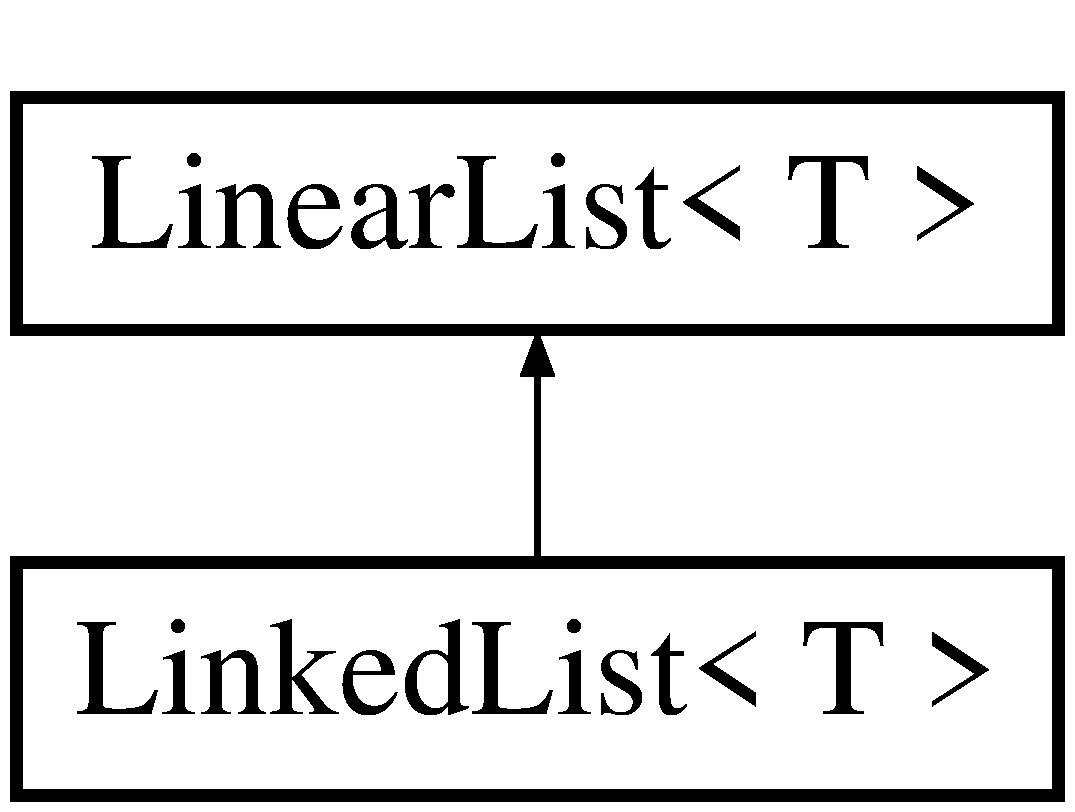
\includegraphics[height=2.000000cm]{classLinkedList}
\end{center}
\end{figure}
\subsection*{Public Member Functions}
\begin{DoxyCompactItemize}
\item 
\mbox{\Hypertarget{classLinkedList_af82224d7ec3e1a5779e9385bf058b6b5}\label{classLinkedList_af82224d7ec3e1a5779e9385bf058b6b5}} 
{\bfseries Linked\+List} (const \hyperlink{classLinkedList}{Linked\+List} \&)
\item 
\mbox{\Hypertarget{classLinkedList_a91a89733b527e2d8eaa08849848be4a5}\label{classLinkedList_a91a89733b527e2d8eaa08849848be4a5}} 
bool {\bfseries empty} () const
\item 
\mbox{\Hypertarget{classLinkedList_aeaa08d2b3584e62dceb5de5e7649fb89}\label{classLinkedList_aeaa08d2b3584e62dceb5de5e7649fb89}} 
int {\bfseries size} () const
\item 
\mbox{\Hypertarget{classLinkedList_a4f0db14e4c550538bba503e90f6db8e8}\label{classLinkedList_a4f0db14e4c550538bba503e90f6db8e8}} 
T \& {\bfseries get} (int) const
\item 
\mbox{\Hypertarget{classLinkedList_a534af13eb6936dfd50ca9bafcc9fab67}\label{classLinkedList_a534af13eb6936dfd50ca9bafcc9fab67}} 
int {\bfseries index\+Of} (const T \&the\+Element) const
\item 
\mbox{\Hypertarget{classLinkedList_abe5bcd829cc8e4f0e9630aa47686aecf}\label{classLinkedList_abe5bcd829cc8e4f0e9630aa47686aecf}} 
void {\bfseries erase} (int the\+Index)
\item 
\mbox{\Hypertarget{classLinkedList_aeebe589f6d8eca4029bde62d71d1a2b8}\label{classLinkedList_aeebe589f6d8eca4029bde62d71d1a2b8}} 
void {\bfseries insert} (int the\+Index, const T \&the\+Element)
\item 
\mbox{\Hypertarget{classLinkedList_a894956b84b369be19134c0bbc72d25bb}\label{classLinkedList_a894956b84b369be19134c0bbc72d25bb}} 
void {\bfseries output} (std\+::ostream \&out) const
\item 
\mbox{\Hypertarget{classLinkedList_a4eb411b244df427dbb5f7ed5374ee2da}\label{classLinkedList_a4eb411b244df427dbb5f7ed5374ee2da}} 
void {\bfseries push\+\_\+back} (const T \&the\+Element)
\end{DoxyCompactItemize}
\subsection*{Protected Member Functions}
\begin{DoxyCompactItemize}
\item 
\mbox{\Hypertarget{classLinkedList_ac780cc43bb96aaad1dafc72a0dc3afcd}\label{classLinkedList_ac780cc43bb96aaad1dafc72a0dc3afcd}} 
void {\bfseries check\+Index} (int the\+Index) const
\end{DoxyCompactItemize}
\subsection*{Protected Attributes}
\begin{DoxyCompactItemize}
\item 
\mbox{\Hypertarget{classLinkedList_aa49a3c2b577167f61868002ca3441019}\label{classLinkedList_aa49a3c2b577167f61868002ca3441019}} 
\hyperlink{structLinkNode}{Link\+Node}$<$ T $>$ $\ast$ {\bfseries header}
\item 
\mbox{\Hypertarget{classLinkedList_adf4e102275c83b4ed732f64ea4c566ee}\label{classLinkedList_adf4e102275c83b4ed732f64ea4c566ee}} 
size\+\_\+t {\bfseries list\+\_\+size}
\end{DoxyCompactItemize}


The documentation for this class was generated from the following file\+:\begin{DoxyCompactItemize}
\item 
data\+\_\+structure/linear\+\_\+list/linked\+\_\+list.\+h\end{DoxyCompactItemize}

\hypertarget{classLinkedStack}{}\section{Linked\+Stack$<$ T $>$ Class Template Reference}
\label{classLinkedStack}\index{Linked\+Stack$<$ T $>$@{Linked\+Stack$<$ T $>$}}
Inheritance diagram for Linked\+Stack$<$ T $>$\+:\begin{figure}[H]
\begin{center}
\leavevmode
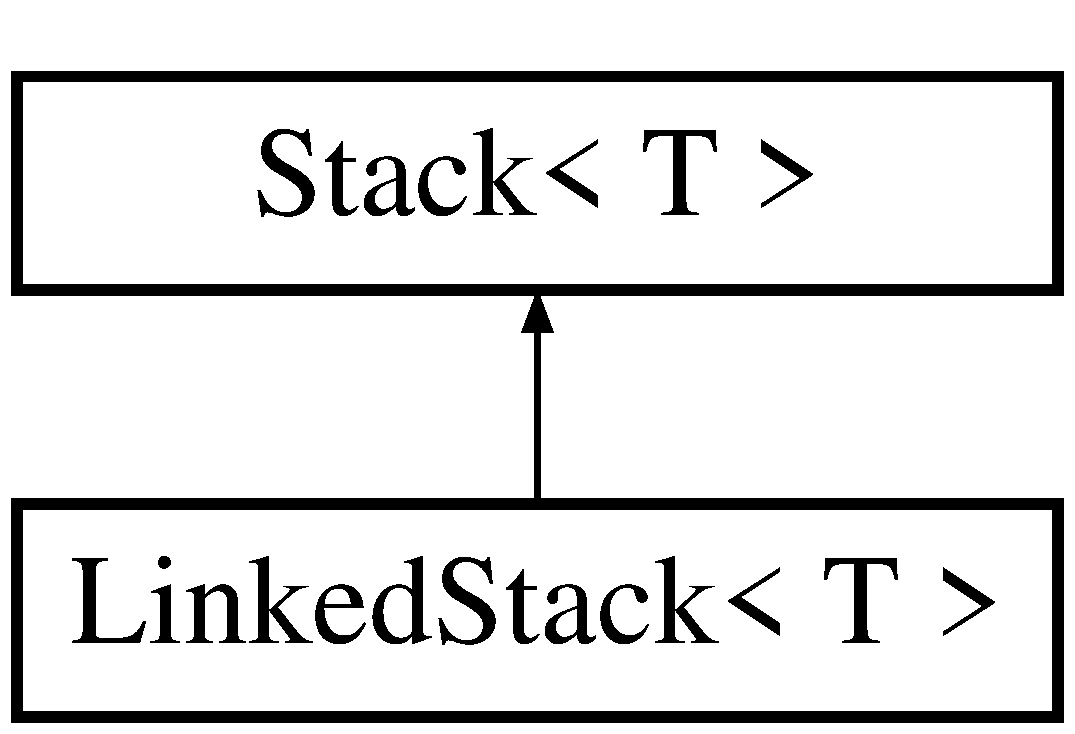
\includegraphics[height=2.000000cm]{classLinkedStack}
\end{center}
\end{figure}
\subsection*{Public Member Functions}
\begin{DoxyCompactItemize}
\item 
\mbox{\Hypertarget{classLinkedStack_a472c529c6991d274634f1c37efc70f55}\label{classLinkedStack_a472c529c6991d274634f1c37efc70f55}} 
bool {\bfseries empty} () const
\item 
\mbox{\Hypertarget{classLinkedStack_a9c57e23fa333a6eb53a3874da556e555}\label{classLinkedStack_a9c57e23fa333a6eb53a3874da556e555}} 
int {\bfseries size} () const
\item 
\mbox{\Hypertarget{classLinkedStack_a6066a454b8361c80f5cd22513a321d8a}\label{classLinkedStack_a6066a454b8361c80f5cd22513a321d8a}} 
T {\bfseries pop} ()
\item 
\mbox{\Hypertarget{classLinkedStack_a1de73e6cfd7c850ef02b8198ffd2ae27}\label{classLinkedStack_a1de73e6cfd7c850ef02b8198ffd2ae27}} 
void {\bfseries push} (const T \&element)
\item 
\mbox{\Hypertarget{classLinkedStack_a62681222006253df75ad12f472d488b7}\label{classLinkedStack_a62681222006253df75ad12f472d488b7}} 
void {\bfseries output} (std\+::ostream \&out) const
\item 
\mbox{\Hypertarget{classLinkedStack_a8407e067813787b24d0570e57988805f}\label{classLinkedStack_a8407e067813787b24d0570e57988805f}} 
T {\bfseries test} ()
\end{DoxyCompactItemize}
\subsection*{Private Attributes}
\begin{DoxyCompactItemize}
\item 
\mbox{\Hypertarget{classLinkedStack_a76b5293e307b263fa9d0eddcb7b1c9fa}\label{classLinkedStack_a76b5293e307b263fa9d0eddcb7b1c9fa}} 
\hyperlink{structLinkNode}{Link\+Node}$<$ T $>$ $\ast$ {\bfseries stack}
\item 
\mbox{\Hypertarget{classLinkedStack_ae2b9dd4011e121427feb00b338d72697}\label{classLinkedStack_ae2b9dd4011e121427feb00b338d72697}} 
int {\bfseries stack\+\_\+size}
\end{DoxyCompactItemize}


The documentation for this class was generated from the following file\+:\begin{DoxyCompactItemize}
\item 
data\+\_\+structure/stack/Linked\+Stack.\+h\end{DoxyCompactItemize}

\hypertarget{structLinkNode}{}\section{Link\+Node$<$ T $>$ Struct Template Reference}
\label{structLinkNode}\index{Link\+Node$<$ T $>$@{Link\+Node$<$ T $>$}}
\subsection*{Public Member Functions}
\begin{DoxyCompactItemize}
\item 
\mbox{\Hypertarget{structLinkNode_ad20c724114b18b55476b507b1a2e232a}\label{structLinkNode_ad20c724114b18b55476b507b1a2e232a}} 
{\bfseries Link\+Node} (const T \&element)
\item 
\mbox{\Hypertarget{structLinkNode_a2a596adde87de51c5f6b03399eab2edc}\label{structLinkNode_a2a596adde87de51c5f6b03399eab2edc}} 
{\bfseries Link\+Node} (const T \&element, \hyperlink{structLinkNode}{Link\+Node}$<$ T $>$ $\ast$next)
\item 
\mbox{\Hypertarget{structLinkNode_a48b62278ea79f7e3c6f1e0d237d54d08}\label{structLinkNode_a48b62278ea79f7e3c6f1e0d237d54d08}} 
{\bfseries Link\+Node} (const \hyperlink{structLinkNode}{Link\+Node} \&node)
\end{DoxyCompactItemize}
\subsection*{Public Attributes}
\begin{DoxyCompactItemize}
\item 
\mbox{\Hypertarget{structLinkNode_ad1ba858aae6858dc555effec6b697faa}\label{structLinkNode_ad1ba858aae6858dc555effec6b697faa}} 
T {\bfseries element}
\item 
\mbox{\Hypertarget{structLinkNode_a19050845bb6742a50b352a3a97e965e2}\label{structLinkNode_a19050845bb6742a50b352a3a97e965e2}} 
\hyperlink{structLinkNode}{Link\+Node} $\ast$ {\bfseries next}
\end{DoxyCompactItemize}


The documentation for this struct was generated from the following file\+:\begin{DoxyCompactItemize}
\item 
data\+\_\+structure/linear\+\_\+list/linked\+\_\+list.\+h\end{DoxyCompactItemize}

\hypertarget{classMaxHblt}{}\section{Max\+Hblt$<$ T $>$ Class Template Reference}
\label{classMaxHblt}\index{Max\+Hblt$<$ T $>$@{Max\+Hblt$<$ T $>$}}
Inheritance diagram for Max\+Hblt$<$ T $>$\+:\begin{figure}[H]
\begin{center}
\leavevmode
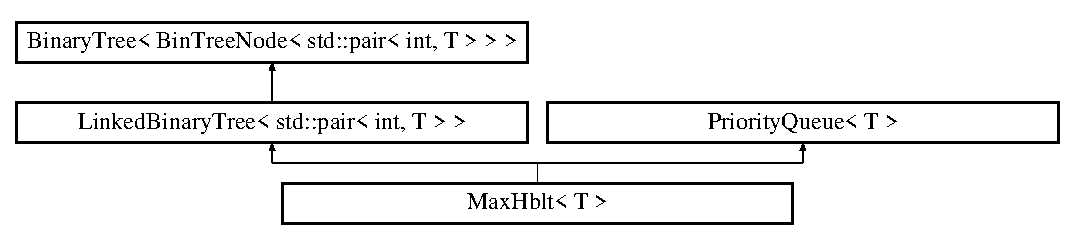
\includegraphics[height=2.781457cm]{classMaxHblt}
\end{center}
\end{figure}
\subsection*{Public Member Functions}
\begin{DoxyCompactItemize}
\item 
\mbox{\Hypertarget{classMaxHblt_ac748ad969d08dd24d4ade6595acd7002}\label{classMaxHblt_ac748ad969d08dd24d4ade6595acd7002}} 
bool \hyperlink{classMaxHblt_ac748ad969d08dd24d4ade6595acd7002}{empty} () const
\begin{DoxyCompactList}\small\item\em if the tree was empty \end{DoxyCompactList}\item 
\mbox{\Hypertarget{classMaxHblt_ae8a4af940e3e9f8f346c63f0407a72cd}\label{classMaxHblt_ae8a4af940e3e9f8f346c63f0407a72cd}} 
size\+\_\+t \hyperlink{classMaxHblt_ae8a4af940e3e9f8f346c63f0407a72cd}{size} () const
\begin{DoxyCompactList}\small\item\em the number of node in thre tree \end{DoxyCompactList}\item 
\mbox{\Hypertarget{classMaxHblt_a70f1601764e0f511357f06e4eed074dc}\label{classMaxHblt_a70f1601764e0f511357f06e4eed074dc}} 
void \hyperlink{classMaxHblt_a70f1601764e0f511357f06e4eed074dc}{meld} (\hyperlink{classMaxHblt}{Max\+Hblt}$<$ T $>$ \&hblt)
\begin{DoxyCompactList}\small\item\em meld two hblt into one \end{DoxyCompactList}\item 
\mbox{\Hypertarget{classMaxHblt_a6c5f2a416535abc326c5e90f7f0f7c3b}\label{classMaxHblt_a6c5f2a416535abc326c5e90f7f0f7c3b}} 
const T \& \hyperlink{classMaxHblt_a6c5f2a416535abc326c5e90f7f0f7c3b}{top} ()
\begin{DoxyCompactList}\small\item\em return the max(min) of the tree \end{DoxyCompactList}\item 
\mbox{\Hypertarget{classMaxHblt_a5941b294086c496fc4eff6e7ebc6b27f}\label{classMaxHblt_a5941b294086c496fc4eff6e7ebc6b27f}} 
T \hyperlink{classMaxHblt_a5941b294086c496fc4eff6e7ebc6b27f}{pop} ()
\begin{DoxyCompactList}\small\item\em pop out the max(min) of thre tree \end{DoxyCompactList}\item 
\mbox{\Hypertarget{classMaxHblt_adfe07cefe42e2a7feddf061a1e601396}\label{classMaxHblt_adfe07cefe42e2a7feddf061a1e601396}} 
void \hyperlink{classMaxHblt_adfe07cefe42e2a7feddf061a1e601396}{push} (const T \&element)
\begin{DoxyCompactList}\small\item\em push a node to the tree \end{DoxyCompactList}\item 
\mbox{\Hypertarget{classMaxHblt_a3f8bd08381873a4fc70e8549130e54e6}\label{classMaxHblt_a3f8bd08381873a4fc70e8549130e54e6}} 
void \hyperlink{classMaxHblt_a3f8bd08381873a4fc70e8549130e54e6}{initialize} (T $\ast$arr, int \hyperlink{classMaxHblt_ae8a4af940e3e9f8f346c63f0407a72cd}{size})
\begin{DoxyCompactList}\small\item\em initialize the maxhblt tree \end{DoxyCompactList}\end{DoxyCompactItemize}
\subsection*{Private Member Functions}
\begin{DoxyCompactItemize}
\item 
void \hyperlink{classMaxHblt_ac60f9c62ad392a8df8bcbd3b91129d37}{meld} (\hyperlink{structBinTreeNode}{Bin\+Tree\+Node}$<$ std\+::pair$<$ int, T $>$$>$ $\ast$\&left, \hyperlink{structBinTreeNode}{Bin\+Tree\+Node}$<$ std\+::pair$<$ int, T $>$$>$ $\ast$\&right)
\end{DoxyCompactItemize}
\subsection*{Additional Inherited Members}


\subsection{Member Function Documentation}
\mbox{\Hypertarget{classMaxHblt_ac60f9c62ad392a8df8bcbd3b91129d37}\label{classMaxHblt_ac60f9c62ad392a8df8bcbd3b91129d37}} 
\index{Max\+Hblt@{Max\+Hblt}!meld@{meld}}
\index{meld@{meld}!Max\+Hblt@{Max\+Hblt}}
\subsubsection{\texorpdfstring{meld()}{meld()}}
{\footnotesize\ttfamily template$<$class T $>$ \\
void \hyperlink{classMaxHblt}{Max\+Hblt}$<$ T $>$\+::meld (\begin{DoxyParamCaption}\item[{\hyperlink{structBinTreeNode}{Bin\+Tree\+Node}$<$ std\+::pair$<$ int, T $>$$>$ $\ast$\&}]{left,  }\item[{\hyperlink{structBinTreeNode}{Bin\+Tree\+Node}$<$ std\+::pair$<$ int, T $>$$>$ $\ast$\&}]{right }\end{DoxyParamCaption})\hspace{0.3cm}{\ttfamily [private]}}

private meld method to recursive call 

The documentation for this class was generated from the following file\+:\begin{DoxyCompactItemize}
\item 
data\+\_\+structure/tree/max\+\_\+hblt.\+h\end{DoxyCompactItemize}

\hypertarget{classMaxHeap}{}\section{Max\+Heap$<$ T $>$ Class Template Reference}
\label{classMaxHeap}\index{Max\+Heap$<$ T $>$@{Max\+Heap$<$ T $>$}}
Inheritance diagram for Max\+Heap$<$ T $>$\+:\begin{figure}[H]
\begin{center}
\leavevmode
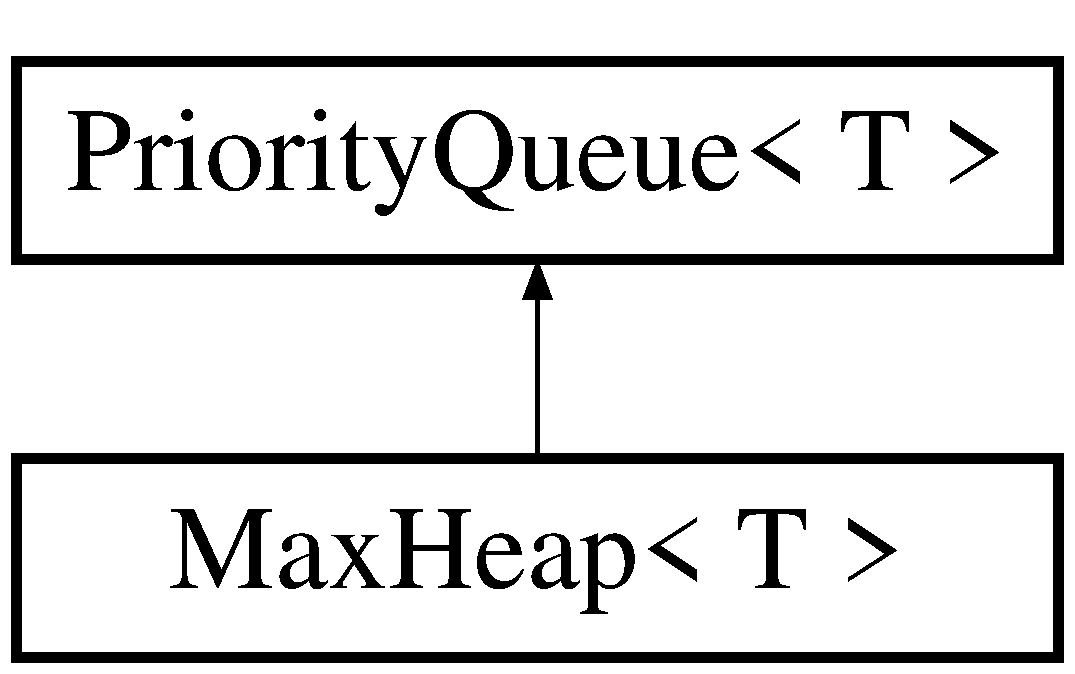
\includegraphics[height=2.000000cm]{classMaxHeap}
\end{center}
\end{figure}
\subsection*{Public Member Functions}
\begin{DoxyCompactItemize}
\item 
\mbox{\Hypertarget{classMaxHeap_a3019a58bae06ffd512751c207ac3a283}\label{classMaxHeap_a3019a58bae06ffd512751c207ac3a283}} 
{\bfseries Max\+Heap} (const \hyperlink{classMaxHeap}{Max\+Heap} \&)
\item 
\mbox{\Hypertarget{classMaxHeap_a69ff7dea02ebd78a83a78c27a2bb9e8e}\label{classMaxHeap_a69ff7dea02ebd78a83a78c27a2bb9e8e}} 
bool {\bfseries empty} () const
\item 
\mbox{\Hypertarget{classMaxHeap_a1894c47131530a277c2f778659520fa4}\label{classMaxHeap_a1894c47131530a277c2f778659520fa4}} 
size\+\_\+t {\bfseries size} () const
\item 
\mbox{\Hypertarget{classMaxHeap_a86d38fba3ad10fadd0f263971789fc59}\label{classMaxHeap_a86d38fba3ad10fadd0f263971789fc59}} 
const T \& {\bfseries top} ()
\item 
\mbox{\Hypertarget{classMaxHeap_a01b465e86ec79b6c920fa6a5d141756b}\label{classMaxHeap_a01b465e86ec79b6c920fa6a5d141756b}} 
T {\bfseries pop} ()
\item 
\mbox{\Hypertarget{classMaxHeap_ada1f7b3a03a4af9dd023ff0f52e92d71}\label{classMaxHeap_ada1f7b3a03a4af9dd023ff0f52e92d71}} 
void {\bfseries push} (const T \&element)
\item 
\mbox{\Hypertarget{classMaxHeap_a0f509a4d2603a54f019e490bceb58858}\label{classMaxHeap_a0f509a4d2603a54f019e490bceb58858}} 
void {\bfseries initialize} (const T $\ast$heap, size\+\_\+t size)
\item 
\mbox{\Hypertarget{classMaxHeap_adb475bbb8add5f39777f83cf982530c2}\label{classMaxHeap_adb475bbb8add5f39777f83cf982530c2}} 
void {\bfseries output} (std\+::ostream \&out) const
\end{DoxyCompactItemize}
\subsection*{Private Member Functions}
\begin{DoxyCompactItemize}
\item 
\mbox{\Hypertarget{classMaxHeap_ab740bb4c5a3b3f922e87c9c8c7b857ef}\label{classMaxHeap_ab740bb4c5a3b3f922e87c9c8c7b857ef}} 
size\+\_\+t {\bfseries max} (size\+\_\+t left, size\+\_\+t right)
\item 
\mbox{\Hypertarget{classMaxHeap_afbbfe6956f66887e8d135acf2bd5a899}\label{classMaxHeap_afbbfe6956f66887e8d135acf2bd5a899}} 
size\+\_\+t {\bfseries max\+\_\+swap} (size\+\_\+t t1, size\+\_\+t t2)
\end{DoxyCompactItemize}
\subsection*{Private Attributes}
\begin{DoxyCompactItemize}
\item 
\mbox{\Hypertarget{classMaxHeap_ad07136d5762b8eaa1b698e194bfd968d}\label{classMaxHeap_ad07136d5762b8eaa1b698e194bfd968d}} 
T $\ast$ {\bfseries heap}
\item 
\mbox{\Hypertarget{classMaxHeap_a266d58512b29a2590ae7c2124abcd8b7}\label{classMaxHeap_a266d58512b29a2590ae7c2124abcd8b7}} 
size\+\_\+t {\bfseries length}
\item 
\mbox{\Hypertarget{classMaxHeap_a75c308a7e7406ddc74242ffbc13e55fd}\label{classMaxHeap_a75c308a7e7406ddc74242ffbc13e55fd}} 
size\+\_\+t {\bfseries heap\+\_\+size}
\end{DoxyCompactItemize}


The documentation for this class was generated from the following file\+:\begin{DoxyCompactItemize}
\item 
data\+\_\+structure/tree/max\+\_\+heap.\+h\end{DoxyCompactItemize}

\hypertarget{classMyIterator}{}\section{My\+Iterator$<$ T $>$ Class Template Reference}
\label{classMyIterator}\index{My\+Iterator$<$ T $>$@{My\+Iterator$<$ T $>$}}
Inheritance diagram for My\+Iterator$<$ T $>$\+:\begin{figure}[H]
\begin{center}
\leavevmode
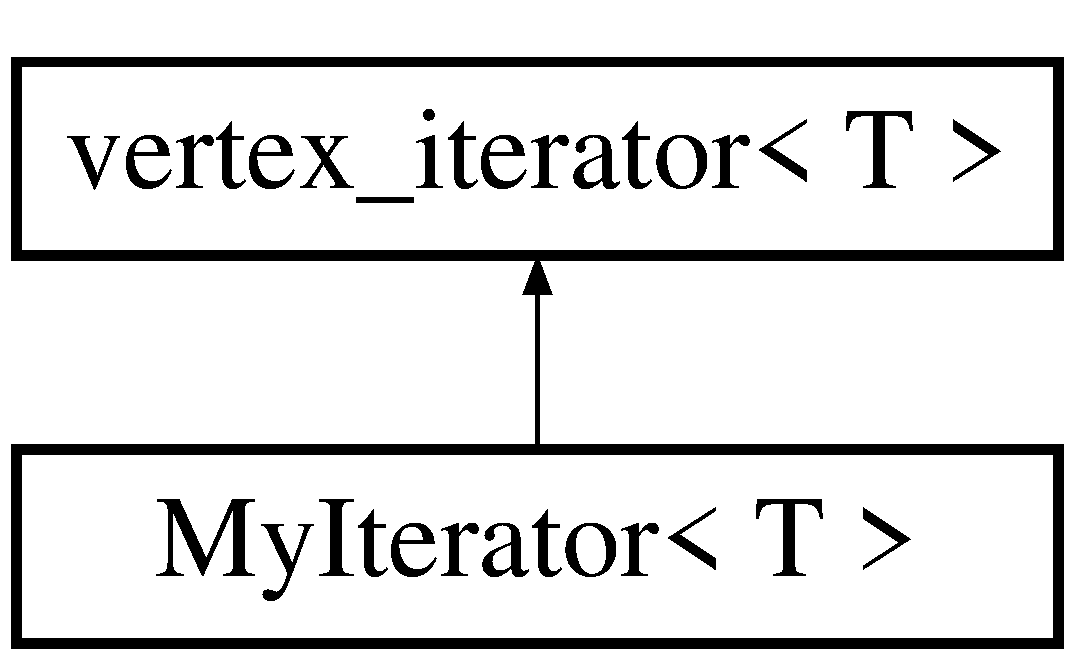
\includegraphics[height=2.000000cm]{classMyIterator}
\end{center}
\end{figure}
\subsection*{Public Member Functions}
\begin{DoxyCompactItemize}
\item 
\mbox{\Hypertarget{classMyIterator_a99709c2c45130a8e6168f5c3bd67be9b}\label{classMyIterator_a99709c2c45130a8e6168f5c3bd67be9b}} 
{\bfseries My\+Iterator} (T $\ast$the\+\_\+row, T the\+\_\+no\+\_\+edge, int num\+\_\+of\+\_\+vertices)
\item 
\mbox{\Hypertarget{classMyIterator_ab77bef399d57de966d653fa1ec124364}\label{classMyIterator_ab77bef399d57de966d653fa1ec124364}} 
int {\bfseries next} (T \&the\+\_\+weight)
\item 
\mbox{\Hypertarget{classMyIterator_ac29886819292cd74b7db18b028d2dcd1}\label{classMyIterator_ac29886819292cd74b7db18b028d2dcd1}} 
int {\bfseries next} ()
\end{DoxyCompactItemize}
\subsection*{Protected Attributes}
\begin{DoxyCompactItemize}
\item 
\mbox{\Hypertarget{classMyIterator_ac2d189e47545152bcfba72e5cb26c1e7}\label{classMyIterator_ac2d189e47545152bcfba72e5cb26c1e7}} 
T $\ast$ {\bfseries row}
\item 
\mbox{\Hypertarget{classMyIterator_a9e27132c6a21661a77f0c572fe7d43e7}\label{classMyIterator_a9e27132c6a21661a77f0c572fe7d43e7}} 
T {\bfseries no\+\_\+edge}
\item 
\mbox{\Hypertarget{classMyIterator_a274bd225f7d1aa8354942ac7b2f8a191}\label{classMyIterator_a274bd225f7d1aa8354942ac7b2f8a191}} 
int {\bfseries n}
\item 
\mbox{\Hypertarget{classMyIterator_ab5eb1cfc4eb8e83362d9d10fd1a7449f}\label{classMyIterator_ab5eb1cfc4eb8e83362d9d10fd1a7449f}} 
int {\bfseries vertex}
\end{DoxyCompactItemize}


The documentation for this class was generated from the following file\+:\begin{DoxyCompactItemize}
\item 
data\+\_\+structure/graph/adj\+\_\+wdigraph.\+h\end{DoxyCompactItemize}

\hypertarget{classPriorityQueue}{}\section{Priority\+Queue$<$ T $>$ Class Template Reference}
\label{classPriorityQueue}\index{Priority\+Queue$<$ T $>$@{Priority\+Queue$<$ T $>$}}
Inheritance diagram for Priority\+Queue$<$ T $>$\+:\begin{figure}[H]
\begin{center}
\leavevmode
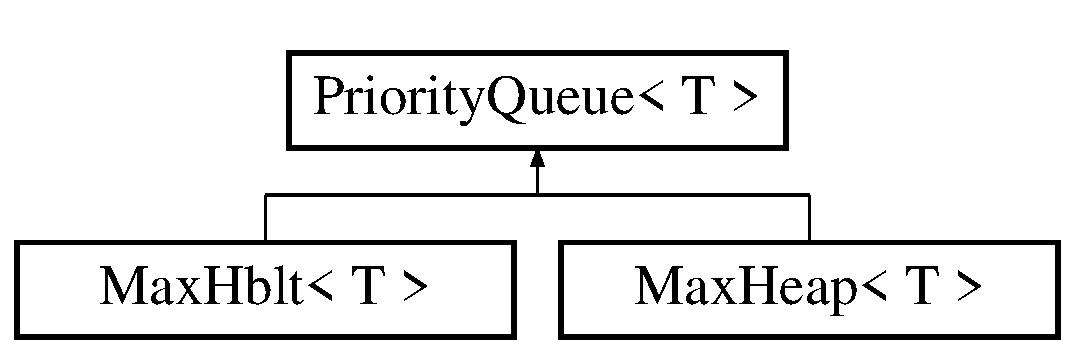
\includegraphics[height=2.000000cm]{classPriorityQueue}
\end{center}
\end{figure}
\subsection*{Public Member Functions}
\begin{DoxyCompactItemize}
\item 
\mbox{\Hypertarget{classPriorityQueue_a8865739774308504e4b1d81c7b385386}\label{classPriorityQueue_a8865739774308504e4b1d81c7b385386}} 
virtual bool {\bfseries empty} () const =0
\item 
\mbox{\Hypertarget{classPriorityQueue_a6ec9a3eaa9e27203bc0d1c5d77f5312a}\label{classPriorityQueue_a6ec9a3eaa9e27203bc0d1c5d77f5312a}} 
virtual size\+\_\+t {\bfseries size} () const =0
\item 
\mbox{\Hypertarget{classPriorityQueue_af3a08e3e21f1ec7abc8f2bb2a4960ee4}\label{classPriorityQueue_af3a08e3e21f1ec7abc8f2bb2a4960ee4}} 
virtual const T \& {\bfseries top} ()=0
\item 
\mbox{\Hypertarget{classPriorityQueue_ad34ccb15bd46775413a8647ccb1af081}\label{classPriorityQueue_ad34ccb15bd46775413a8647ccb1af081}} 
virtual T {\bfseries pop} ()=0
\item 
\mbox{\Hypertarget{classPriorityQueue_abfa3615ae45c98a2744b23b895fa7df1}\label{classPriorityQueue_abfa3615ae45c98a2744b23b895fa7df1}} 
virtual void {\bfseries push} (const T \&element)=0
\end{DoxyCompactItemize}


The documentation for this class was generated from the following file\+:\begin{DoxyCompactItemize}
\item 
data\+\_\+structure/tree/priority\+\_\+queue.\+h\end{DoxyCompactItemize}

\hypertarget{classQueue}{}\section{Queue$<$ T $>$ Class Template Reference}
\label{classQueue}\index{Queue$<$ T $>$@{Queue$<$ T $>$}}
Inheritance diagram for Queue$<$ T $>$\+:\begin{figure}[H]
\begin{center}
\leavevmode
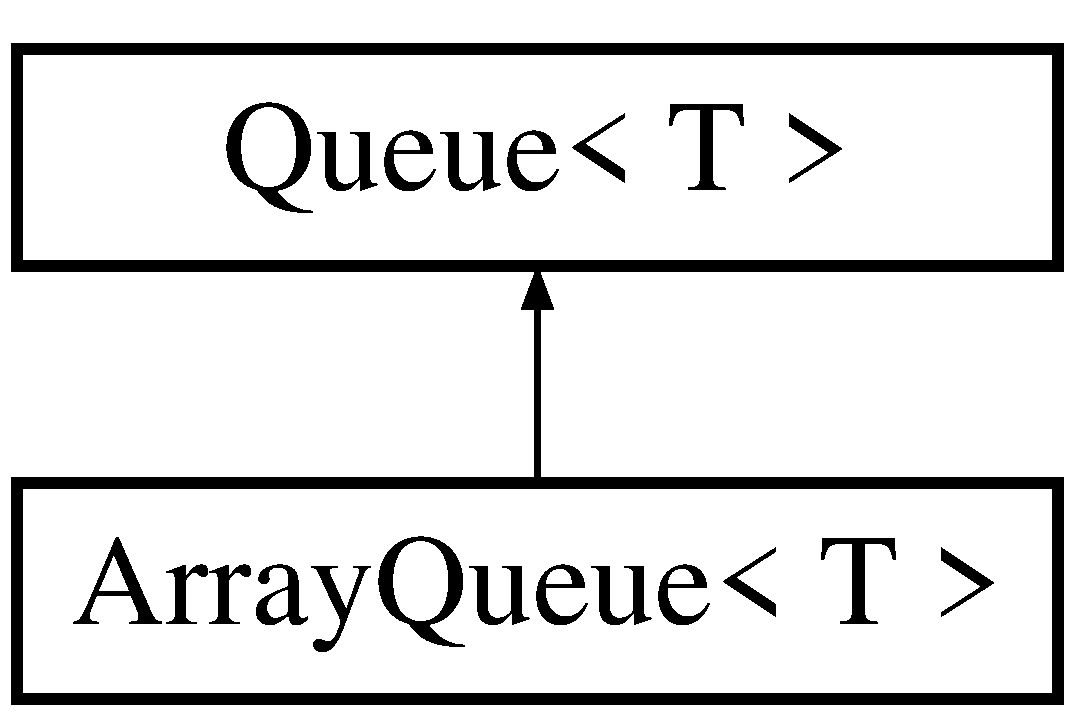
\includegraphics[height=2.000000cm]{classQueue}
\end{center}
\end{figure}
\subsection*{Public Member Functions}
\begin{DoxyCompactItemize}
\item 
\mbox{\Hypertarget{classQueue_a5b1556252d112e340c96b73f1e5a9836}\label{classQueue_a5b1556252d112e340c96b73f1e5a9836}} 
virtual bool {\bfseries empty} () const =0
\item 
\mbox{\Hypertarget{classQueue_a57c59f0de878241b175803359b1da05e}\label{classQueue_a57c59f0de878241b175803359b1da05e}} 
virtual int {\bfseries size} () const =0
\item 
\mbox{\Hypertarget{classQueue_af0901eae22d8c66141e114b45392ec32}\label{classQueue_af0901eae22d8c66141e114b45392ec32}} 
virtual T \& {\bfseries front} ()=0
\item 
\mbox{\Hypertarget{classQueue_a32e02644d90c190c69fb693c81fc3237}\label{classQueue_a32e02644d90c190c69fb693c81fc3237}} 
virtual T \& {\bfseries back} ()=0
\item 
\mbox{\Hypertarget{classQueue_a6c162a551ebcdc53e53d6895aac541c1}\label{classQueue_a6c162a551ebcdc53e53d6895aac541c1}} 
virtual T {\bfseries pop} ()=0
\item 
\mbox{\Hypertarget{classQueue_a8fa3be99d4c44e7b439327a37b4b23c9}\label{classQueue_a8fa3be99d4c44e7b439327a37b4b23c9}} 
virtual void {\bfseries push} (const T \&element)=0
\end{DoxyCompactItemize}


The documentation for this class was generated from the following file\+:\begin{DoxyCompactItemize}
\item 
data\+\_\+structure/queue/queue.\+h\end{DoxyCompactItemize}

\hypertarget{structRBTreeNode}{}\section{R\+B\+Tree\+Node$<$ T $>$ Struct Template Reference}
\label{structRBTreeNode}\index{R\+B\+Tree\+Node$<$ T $>$@{R\+B\+Tree\+Node$<$ T $>$}}
\subsection*{Public Member Functions}
\begin{DoxyCompactItemize}
\item 
\mbox{\Hypertarget{structRBTreeNode_aae4119573b6ce9f44289cbeaa225775a}\label{structRBTreeNode_aae4119573b6ce9f44289cbeaa225775a}} 
{\bfseries R\+B\+Tree\+Node} (const T \&t)
\item 
\mbox{\Hypertarget{structRBTreeNode_a753595687f5adeef15b0b08813d86023}\label{structRBTreeNode_a753595687f5adeef15b0b08813d86023}} 
{\bfseries R\+B\+Tree\+Node} (const \hyperlink{structRBTreeNode}{R\+B\+Tree\+Node} \&node)
\item 
\mbox{\Hypertarget{structRBTreeNode_a3623d833c4682c8a6b7437ae8e6bd1c9}\label{structRBTreeNode_a3623d833c4682c8a6b7437ae8e6bd1c9}} 
{\bfseries R\+B\+Tree\+Node} (const T element, \hyperlink{structRBTreeNode}{R\+B\+Tree\+Node}$<$ T $>$ $\ast$left, \hyperlink{structRBTreeNode}{R\+B\+Tree\+Node}$<$ T $>$ $\ast$right, \hyperlink{structRBTreeNode}{R\+B\+Tree\+Node}$<$ T $>$ $\ast$p)
\item 
\mbox{\Hypertarget{structRBTreeNode_a11f770591252473508eea8ad1b6dff55}\label{structRBTreeNode_a11f770591252473508eea8ad1b6dff55}} 
{\bfseries R\+B\+Tree\+Node} (const T element, \hyperlink{structRBTreeNode}{R\+B\+Tree\+Node}$<$ T $>$ $\ast$left, \hyperlink{structRBTreeNode}{R\+B\+Tree\+Node}$<$ T $>$ $\ast$right, \hyperlink{structRBTreeNode}{R\+B\+Tree\+Node}$<$ T $>$ $\ast$p, C\+O\+L\+OR color)
\end{DoxyCompactItemize}
\subsection*{Public Attributes}
\begin{DoxyCompactItemize}
\item 
\mbox{\Hypertarget{structRBTreeNode_a66086a6ccff375f485d447836fe5c97c}\label{structRBTreeNode_a66086a6ccff375f485d447836fe5c97c}} 
T {\bfseries element}
\item 
\mbox{\Hypertarget{structRBTreeNode_a9a848dad720599a9669b3eefbfe6f258}\label{structRBTreeNode_a9a848dad720599a9669b3eefbfe6f258}} 
\hyperlink{structRBTreeNode}{R\+B\+Tree\+Node}$<$ T $>$ $\ast$ {\bfseries left}
\item 
\mbox{\Hypertarget{structRBTreeNode_aebfeee7f7a5e16bc302a0c4973c2f3ed}\label{structRBTreeNode_aebfeee7f7a5e16bc302a0c4973c2f3ed}} 
\hyperlink{structRBTreeNode}{R\+B\+Tree\+Node}$<$ T $>$ $\ast$ {\bfseries right}
\item 
\mbox{\Hypertarget{structRBTreeNode_a8dbffe97c5d8402b59eb653b2598c1c0}\label{structRBTreeNode_a8dbffe97c5d8402b59eb653b2598c1c0}} 
\hyperlink{structRBTreeNode}{R\+B\+Tree\+Node}$<$ T $>$ $\ast$ {\bfseries p}
\item 
\mbox{\Hypertarget{structRBTreeNode_a68e427bce0961318d678c47a8ac706a5}\label{structRBTreeNode_a68e427bce0961318d678c47a8ac706a5}} 
C\+O\+L\+OR {\bfseries color}
\end{DoxyCompactItemize}
\subsection*{Static Public Attributes}
\begin{DoxyCompactItemize}
\item 
\mbox{\Hypertarget{structRBTreeNode_aaf39e40ebd40db6ed1493b6ae262dc9d}\label{structRBTreeNode_aaf39e40ebd40db6ed1493b6ae262dc9d}} 
static \hyperlink{structRBTreeNode}{R\+B\+Tree\+Node} $\ast$ {\bfseries nil} = new \hyperlink{structRBTreeNode}{R\+B\+Tree\+Node}$<$T$>$()
\end{DoxyCompactItemize}


The documentation for this struct was generated from the following file\+:\begin{DoxyCompactItemize}
\item 
data\+\_\+structure/tree/tree\+\_\+p/rb\+\_\+tree\+\_\+node.\+h\end{DoxyCompactItemize}

\hypertarget{classRedBlackTree}{}\section{Red\+Black\+Tree$<$ K, E $>$ Class Template Reference}
\label{classRedBlackTree}\index{Red\+Black\+Tree$<$ K, E $>$@{Red\+Black\+Tree$<$ K, E $>$}}
Inheritance diagram for Red\+Black\+Tree$<$ K, E $>$\+:\begin{figure}[H]
\begin{center}
\leavevmode
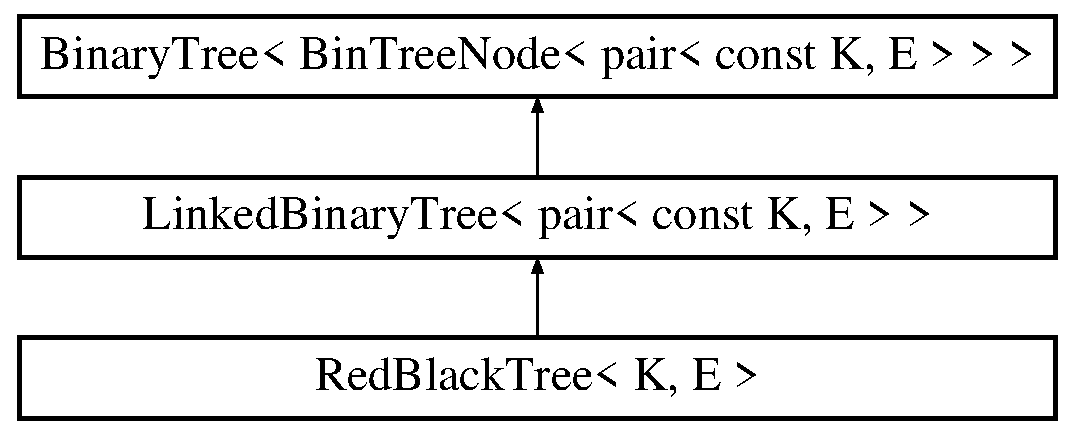
\includegraphics[height=3.000000cm]{classRedBlackTree}
\end{center}
\end{figure}
\subsection*{Public Types}
\begin{DoxyCompactItemize}
\item 
\mbox{\Hypertarget{classRedBlackTree_aa066ea6a55f097b0ddc01f92217ca4b3}\label{classRedBlackTree_aa066ea6a55f097b0ddc01f92217ca4b3}} 
typedef \hyperlink{structRBTreeNode}{R\+B\+Tree\+Node}$<$ pair$<$ const K, E $>$ $>$ {\bfseries Node}
\end{DoxyCompactItemize}
\subsection*{Public Member Functions}
\begin{DoxyCompactItemize}
\item 
\mbox{\Hypertarget{classRedBlackTree_a22a9b5fe5f5792160163fc68d3a72364}\label{classRedBlackTree_a22a9b5fe5f5792160163fc68d3a72364}} 
const pair$<$ const K, E $>$ \& {\bfseries search} (const K \&) const
\item 
\mbox{\Hypertarget{classRedBlackTree_aa57aaacc1bb547efd1eeea3449de57c3}\label{classRedBlackTree_aa57aaacc1bb547efd1eeea3449de57c3}} 
\hyperlink{structRBTreeNode}{Node} $\ast$const {\bfseries minimum} () const
\item 
\mbox{\Hypertarget{classRedBlackTree_a108f44497081568d03f7533a5ba8dbb3}\label{classRedBlackTree_a108f44497081568d03f7533a5ba8dbb3}} 
\hyperlink{structRBTreeNode}{Node} $\ast$const {\bfseries maximum} () const
\item 
\mbox{\Hypertarget{classRedBlackTree_ab81e72ce029c6e240960c259bd070d6a}\label{classRedBlackTree_ab81e72ce029c6e240960c259bd070d6a}} 
const pair$<$ const K, E $>$ \& {\bfseries successor} (const K \&) const
\item 
\mbox{\Hypertarget{classRedBlackTree_a279825b0f6c710e4e7797b5987d4d948}\label{classRedBlackTree_a279825b0f6c710e4e7797b5987d4d948}} 
const pair$<$ const K, E $>$ \& {\bfseries predecessor} (const K \&) const
\item 
\mbox{\Hypertarget{classRedBlackTree_a87d6a25ba6d6b77344870b8fd50765d3}\label{classRedBlackTree_a87d6a25ba6d6b77344870b8fd50765d3}} 
void {\bfseries insert} (const pair$<$ const K, E $>$ \&)
\item 
\mbox{\Hypertarget{classRedBlackTree_a926cd4e9c05210789e03663dd5148a9b}\label{classRedBlackTree_a926cd4e9c05210789e03663dd5148a9b}} 
void {\bfseries tree\+\_\+delete} (const K \&)
\end{DoxyCompactItemize}
\subsection*{Private Member Functions}
\begin{DoxyCompactItemize}
\item 
\mbox{\Hypertarget{classRedBlackTree_a6a3c5b202fdaee39152a185c6fc4a3c0}\label{classRedBlackTree_a6a3c5b202fdaee39152a185c6fc4a3c0}} 
\hyperlink{structRBTreeNode}{Node} $\ast$const {\bfseries minimum} (\hyperlink{structRBTreeNode}{Node} $\ast$) const
\item 
\mbox{\Hypertarget{classRedBlackTree_a95ada18cc67ea0bcdd25b816dcf8cd4e}\label{classRedBlackTree_a95ada18cc67ea0bcdd25b816dcf8cd4e}} 
\hyperlink{structRBTreeNode}{Node} $\ast$const {\bfseries maximum} (\hyperlink{structRBTreeNode}{Node} $\ast$) const
\item 
\mbox{\Hypertarget{classRedBlackTree_a06dce17014728689d32e4e0cbbce3685}\label{classRedBlackTree_a06dce17014728689d32e4e0cbbce3685}} 
void {\bfseries transplant} (\hyperlink{structRBTreeNode}{Node} $\ast$, \hyperlink{structRBTreeNode}{Node} $\ast$)
\item 
\mbox{\Hypertarget{classRedBlackTree_a15b709e0fe1adf23f6adb22f17401013}\label{classRedBlackTree_a15b709e0fe1adf23f6adb22f17401013}} 
\hyperlink{structRBTreeNode}{Node} $\ast$ {\bfseries find} (const K \&key) const
\item 
\mbox{\Hypertarget{classRedBlackTree_a014683afc23d8cb321cb44b4edc442a4}\label{classRedBlackTree_a014683afc23d8cb321cb44b4edc442a4}} 
void {\bfseries left\+\_\+rotate} (\hyperlink{structRBTreeNode}{Node} $\ast$)
\item 
\mbox{\Hypertarget{classRedBlackTree_a7f9850af2258827381214b5eb46b3ebb}\label{classRedBlackTree_a7f9850af2258827381214b5eb46b3ebb}} 
void {\bfseries right\+\_\+rotate} (\hyperlink{structRBTreeNode}{Node} $\ast$)
\item 
\mbox{\Hypertarget{classRedBlackTree_a245c2d25489e65d31df086af17fabbc0}\label{classRedBlackTree_a245c2d25489e65d31df086af17fabbc0}} 
void {\bfseries insert\+\_\+fixup} (\hyperlink{structRBTreeNode}{Node} $\ast$)
\item 
\mbox{\Hypertarget{classRedBlackTree_a9d70e240c81ba402cce60b04fed92309}\label{classRedBlackTree_a9d70e240c81ba402cce60b04fed92309}} 
void {\bfseries delete\+\_\+fixup} (\hyperlink{structRBTreeNode}{Node} $\ast$)
\end{DoxyCompactItemize}
\subsection*{Additional Inherited Members}


The documentation for this class was generated from the following file\+:\begin{DoxyCompactItemize}
\item 
data\+\_\+structure/tree/tree\+\_\+p/red\+\_\+black\+\_\+tree.\+h\end{DoxyCompactItemize}

\hypertarget{classServer}{}\section{Server Class Reference}
\label{classServer}\index{Server@{Server}}
\subsection*{Public Types}
\begin{DoxyCompactItemize}
\item 
\mbox{\Hypertarget{classServer_a1704a3918f1a1d44f4f7ad8223ddfdc8}\label{classServer_a1704a3918f1a1d44f4f7ad8223ddfdc8}} 
typedef std\+::shared\+\_\+ptr$<$ ip\+::tcp\+::socket $>$ {\bfseries socket\+\_\+ptr}
\end{DoxyCompactItemize}
\subsection*{Public Member Functions}
\begin{DoxyCompactItemize}
\item 
\mbox{\Hypertarget{classServer_a4df8b0535563c8ed3ff6d61b734a1f78}\label{classServer_a4df8b0535563c8ed3ff6d61b734a1f78}} 
{\bfseries Server} (io\+\_\+service \&ser)
\item 
\mbox{\Hypertarget{classServer_a7eac07d2582fa01c2671362efa955b31}\label{classServer_a7eac07d2582fa01c2671362efa955b31}} 
void {\bfseries start} ()
\end{DoxyCompactItemize}
\subsection*{Protected Member Functions}
\begin{DoxyCompactItemize}
\item 
\mbox{\Hypertarget{classServer_afc6b790ef64c0ce37330a7d2d1d6ccd5}\label{classServer_afc6b790ef64c0ce37330a7d2d1d6ccd5}} 
void {\bfseries start\+\_\+accept} (socket\+\_\+ptr psocket)
\item 
\mbox{\Hypertarget{classServer_a3468a5afb9b04ac93f4c157f74d12640}\label{classServer_a3468a5afb9b04ac93f4c157f74d12640}} 
void {\bfseries handle\+\_\+accept} (socket\+\_\+ptr psocket, const boost\+::system\+::error\+\_\+code ec)
\end{DoxyCompactItemize}
\subsection*{Protected Attributes}
\begin{DoxyCompactItemize}
\item 
\mbox{\Hypertarget{classServer_ae4722c2f98948cc7c2c672b32d3c553e}\label{classServer_ae4722c2f98948cc7c2c672b32d3c553e}} 
io\+\_\+service \& {\bfseries service}
\item 
\mbox{\Hypertarget{classServer_ae847c95edf67fb1625f1ed7b2936fc6e}\label{classServer_ae847c95edf67fb1625f1ed7b2936fc6e}} 
ip\+::tcp\+::endpoint {\bfseries ep}
\item 
\mbox{\Hypertarget{classServer_a3b3f2b34d9778274dde9c4cbf2d2d9f4}\label{classServer_a3b3f2b34d9778274dde9c4cbf2d2d9f4}} 
ip\+::tcp\+::acceptor {\bfseries ac}
\end{DoxyCompactItemize}


The documentation for this class was generated from the following file\+:\begin{DoxyCompactItemize}
\item 
asio/async\+\_\+server.\+cc\end{DoxyCompactItemize}

\hypertarget{classStack}{}\section{Stack$<$ T $>$ Class Template Reference}
\label{classStack}\index{Stack$<$ T $>$@{Stack$<$ T $>$}}
Inheritance diagram for Stack$<$ T $>$\+:\begin{figure}[H]
\begin{center}
\leavevmode
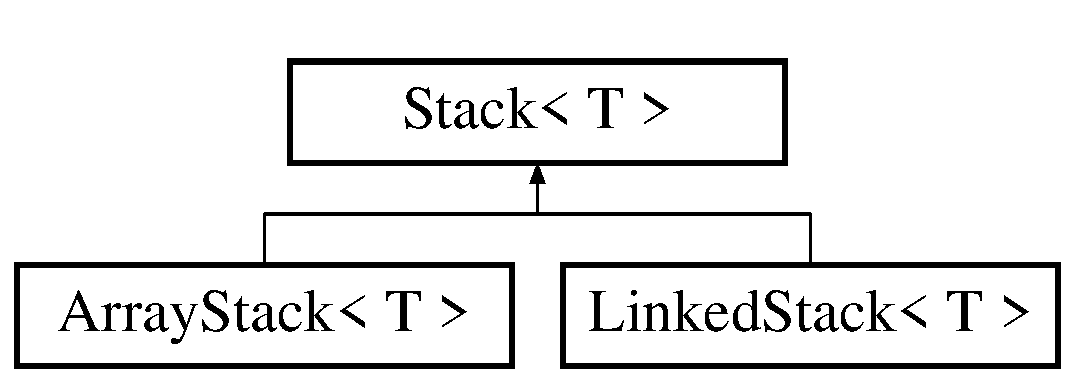
\includegraphics[height=2.000000cm]{classStack}
\end{center}
\end{figure}
\subsection*{Public Member Functions}
\begin{DoxyCompactItemize}
\item 
\mbox{\Hypertarget{classStack_afbfc6378d9b9381137f0dd59943c8eae}\label{classStack_afbfc6378d9b9381137f0dd59943c8eae}} 
virtual bool {\bfseries empty} () const =0
\item 
\mbox{\Hypertarget{classStack_a476b1b8ab66ea042d669eebdc81568ec}\label{classStack_a476b1b8ab66ea042d669eebdc81568ec}} 
virtual int {\bfseries size} () const =0
\item 
\mbox{\Hypertarget{classStack_afae3a6ed7acb65919b802991ccbdd4cd}\label{classStack_afae3a6ed7acb65919b802991ccbdd4cd}} 
virtual T {\bfseries pop} ()=0
\item 
\mbox{\Hypertarget{classStack_a5fde93daf38b1c1579c208ed411e664c}\label{classStack_a5fde93daf38b1c1579c208ed411e664c}} 
virtual void {\bfseries push} (const T \&element)=0
\end{DoxyCompactItemize}


The documentation for this class was generated from the following file\+:\begin{DoxyCompactItemize}
\item 
data\+\_\+structure/stack/stack.\+h\end{DoxyCompactItemize}

\hypertarget{classVectorList}{}\section{Vector\+List$<$ T $>$ Class Template Reference}
\label{classVectorList}\index{Vector\+List$<$ T $>$@{Vector\+List$<$ T $>$}}
Inheritance diagram for Vector\+List$<$ T $>$\+:\begin{figure}[H]
\begin{center}
\leavevmode
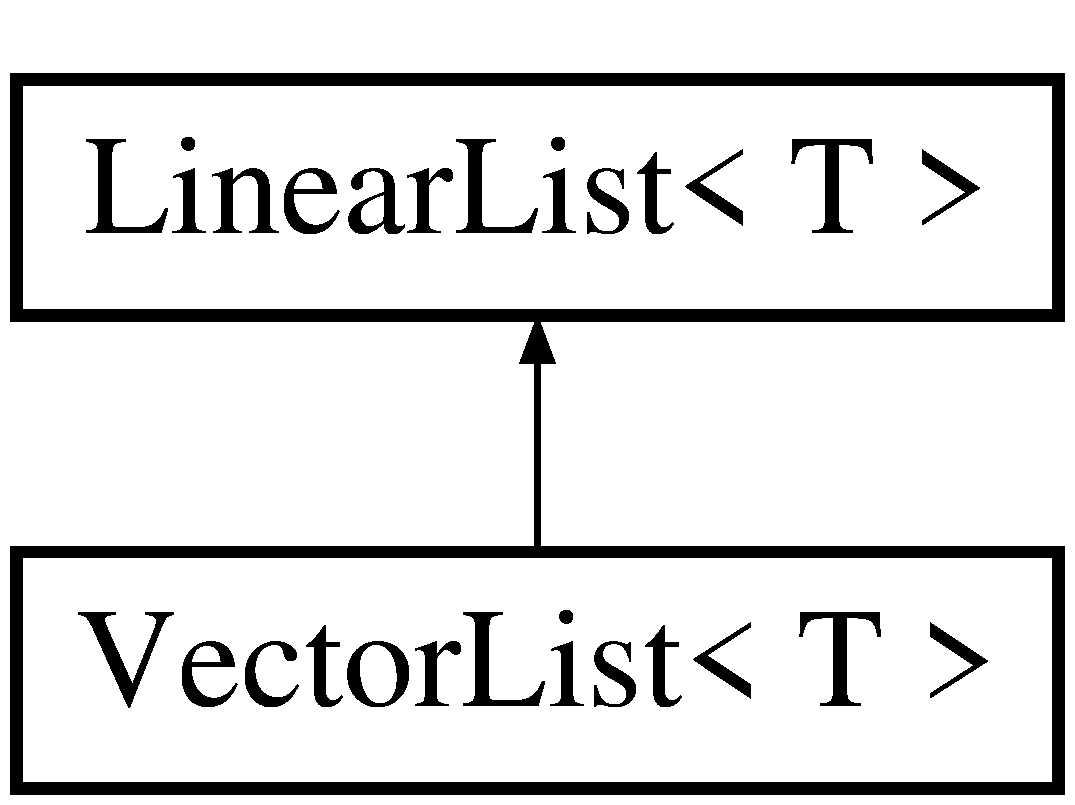
\includegraphics[height=2.000000cm]{classVectorList}
\end{center}
\end{figure}
\subsection*{Public Types}
\begin{DoxyCompactItemize}
\item 
\mbox{\Hypertarget{classVectorList_a9aa89b0156dca1ebe731f2296e7a5e38}\label{classVectorList_a9aa89b0156dca1ebe731f2296e7a5e38}} 
typedef std\+::vector$<$ T $>$\+::\hyperlink{classiterator}{iterator} {\bfseries iterator}
\end{DoxyCompactItemize}
\subsection*{Public Member Functions}
\begin{DoxyCompactItemize}
\item 
\mbox{\Hypertarget{classVectorList_a125d5866d0d98b696c996d9f4b7d87af}\label{classVectorList_a125d5866d0d98b696c996d9f4b7d87af}} 
{\bfseries Vector\+List} (int length=10)
\item 
\mbox{\Hypertarget{classVectorList_a5fa6e7518053eba69818ec99acb92a71}\label{classVectorList_a5fa6e7518053eba69818ec99acb92a71}} 
{\bfseries Vector\+List} (const \hyperlink{classVectorList}{Vector\+List}$<$ T $>$ \&)
\item 
\mbox{\Hypertarget{classVectorList_a7ba6e916d1d9f0f3c3b73883eaf9fc9a}\label{classVectorList_a7ba6e916d1d9f0f3c3b73883eaf9fc9a}} 
bool {\bfseries empty} () const
\item 
\mbox{\Hypertarget{classVectorList_a914cc0d95c50c2525e72dc61cb5b86c7}\label{classVectorList_a914cc0d95c50c2525e72dc61cb5b86c7}} 
int {\bfseries size} () const
\item 
\mbox{\Hypertarget{classVectorList_a3f2d17e63ce64a5cd32c4283544779d8}\label{classVectorList_a3f2d17e63ce64a5cd32c4283544779d8}} 
T \& {\bfseries get} (int the\+Index) const
\item 
\mbox{\Hypertarget{classVectorList_a1cc6db97a3a9abee9f2d6d002695f1a9}\label{classVectorList_a1cc6db97a3a9abee9f2d6d002695f1a9}} 
int {\bfseries index\+Of} (const T \&the\+Element) const
\item 
\mbox{\Hypertarget{classVectorList_ad6aa0bb07676f23de797dfa9ba4f3d7b}\label{classVectorList_ad6aa0bb07676f23de797dfa9ba4f3d7b}} 
void {\bfseries erase} (int the\+Index)
\item 
\mbox{\Hypertarget{classVectorList_ad64994fce0685742e46e3b27d4dd6d40}\label{classVectorList_ad64994fce0685742e46e3b27d4dd6d40}} 
void {\bfseries insert} (int the\+Index, const T \&the\+Element)
\item 
\mbox{\Hypertarget{classVectorList_aa65ee0290429edf9fb1566880df23704}\label{classVectorList_aa65ee0290429edf9fb1566880df23704}} 
void {\bfseries output} (std\+::ostream \&out) const
\item 
\mbox{\Hypertarget{classVectorList_a4c51e98c987b77b6c76476f5d6cddcd6}\label{classVectorList_a4c51e98c987b77b6c76476f5d6cddcd6}} 
void {\bfseries push\+\_\+back} (const T \&the\+Element)
\item 
\mbox{\Hypertarget{classVectorList_ae62bab6c720f860f4eda0d4b4ea1f629}\label{classVectorList_ae62bab6c720f860f4eda0d4b4ea1f629}} 
int {\bfseries capacity} () const
\item 
\mbox{\Hypertarget{classVectorList_ada561e1f71ba030f89638ecc86576724}\label{classVectorList_ada561e1f71ba030f89638ecc86576724}} 
\hyperlink{classiterator}{iterator} {\bfseries begin} ()
\item 
\mbox{\Hypertarget{classVectorList_af568c506954c234b8dcbdc2ee9846e47}\label{classVectorList_af568c506954c234b8dcbdc2ee9846e47}} 
\hyperlink{classiterator}{iterator} {\bfseries end} ()
\end{DoxyCompactItemize}
\subsection*{Protected Member Functions}
\begin{DoxyCompactItemize}
\item 
\mbox{\Hypertarget{classVectorList_adf7ba2201d2f8fb3b85e7ba2bdd04e14}\label{classVectorList_adf7ba2201d2f8fb3b85e7ba2bdd04e14}} 
void {\bfseries check\+Index} (int the\+Index) const
\end{DoxyCompactItemize}
\subsection*{Protected Attributes}
\begin{DoxyCompactItemize}
\item 
\mbox{\Hypertarget{classVectorList_a5e800cced373d2fe09c57ec9ef128004}\label{classVectorList_a5e800cced373d2fe09c57ec9ef128004}} 
std\+::vector$<$ T $>$ $\ast$ {\bfseries element}
\end{DoxyCompactItemize}


The documentation for this class was generated from the following file\+:\begin{DoxyCompactItemize}
\item 
data\+\_\+structure/linear\+\_\+list/vector\+\_\+list.\+h\end{DoxyCompactItemize}

\hypertarget{classvertex__iterator}{}\section{vertex\+\_\+iterator$<$ T $>$ Class Template Reference}
\label{classvertex__iterator}\index{vertex\+\_\+iterator$<$ T $>$@{vertex\+\_\+iterator$<$ T $>$}}
Inheritance diagram for vertex\+\_\+iterator$<$ T $>$\+:\begin{figure}[H]
\begin{center}
\leavevmode
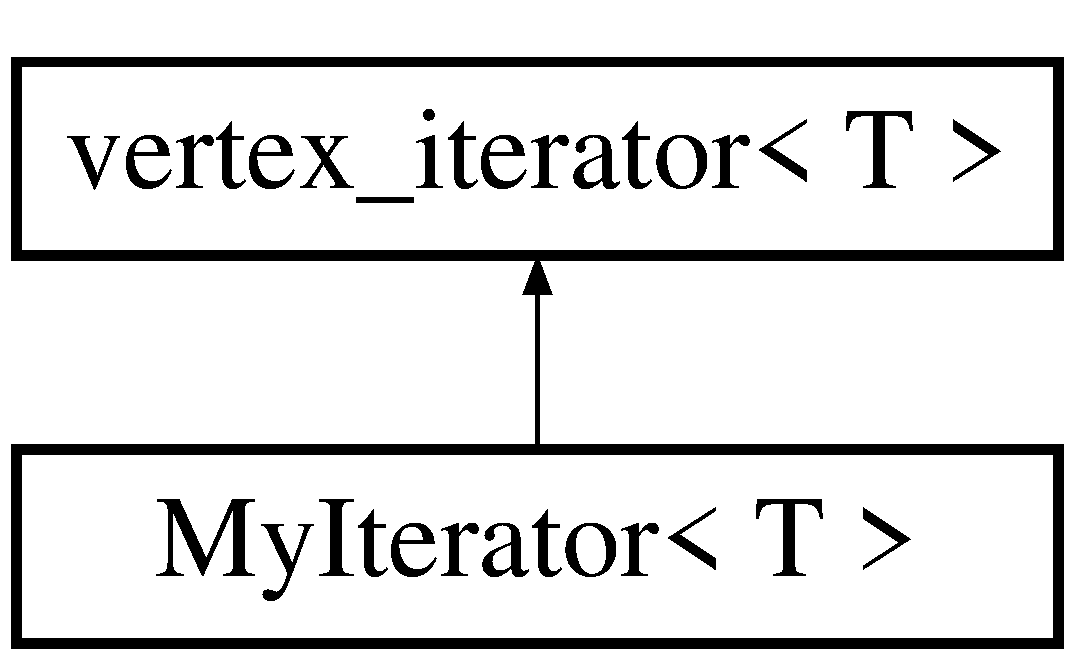
\includegraphics[height=2.000000cm]{classvertex__iterator}
\end{center}
\end{figure}
\subsection*{Public Member Functions}
\begin{DoxyCompactItemize}
\item 
\mbox{\Hypertarget{classvertex__iterator_a451193f6cf58f363602cf92e9757b85d}\label{classvertex__iterator_a451193f6cf58f363602cf92e9757b85d}} 
virtual int {\bfseries next} ()=0
\item 
\mbox{\Hypertarget{classvertex__iterator_ae3179a8bcb5f3cb4c021d79a029fd867}\label{classvertex__iterator_ae3179a8bcb5f3cb4c021d79a029fd867}} 
virtual int {\bfseries next} (T \&)=0
\end{DoxyCompactItemize}


The documentation for this class was generated from the following file\+:\begin{DoxyCompactItemize}
\item 
data\+\_\+structure/graph/graph.\+h\end{DoxyCompactItemize}

\hypertarget{classWinnerTree}{}\section{Winner\+Tree$<$ T $>$ Class Template Reference}
\label{classWinnerTree}\index{Winner\+Tree$<$ T $>$@{Winner\+Tree$<$ T $>$}}
Inheritance diagram for Winner\+Tree$<$ T $>$\+:\begin{figure}[H]
\begin{center}
\leavevmode
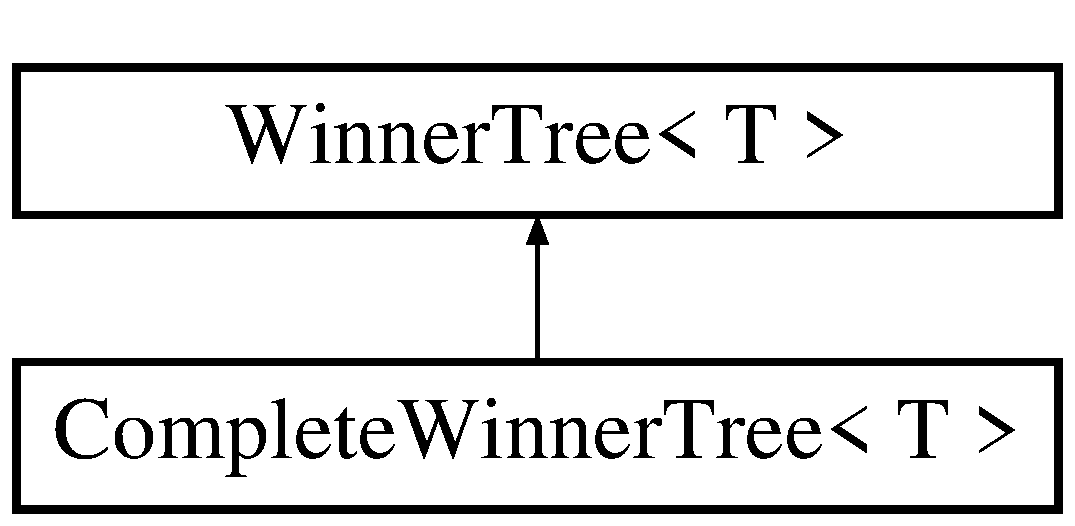
\includegraphics[height=2.000000cm]{classWinnerTree}
\end{center}
\end{figure}
\subsection*{Public Member Functions}
\begin{DoxyCompactItemize}
\item 
\mbox{\Hypertarget{classWinnerTree_af1065e5749f146aa8e8e2321f2c62bbd}\label{classWinnerTree_af1065e5749f146aa8e8e2321f2c62bbd}} 
virtual void {\bfseries initialize} (T $\ast$, int)=0
\item 
\mbox{\Hypertarget{classWinnerTree_a29bc74be01f7bb92452248e7dc2e02cb}\label{classWinnerTree_a29bc74be01f7bb92452248e7dc2e02cb}} 
virtual size\+\_\+t {\bfseries winner} ()=0
\item 
\mbox{\Hypertarget{classWinnerTree_a230bbd5dfd5a8a184bddc2e5937ceba3}\label{classWinnerTree_a230bbd5dfd5a8a184bddc2e5937ceba3}} 
virtual void {\bfseries replay} (size\+\_\+t player)=0
\end{DoxyCompactItemize}


The documentation for this class was generated from the following file\+:\begin{DoxyCompactItemize}
\item 
data\+\_\+structure/tree/winner\+\_\+tree.\+h\end{DoxyCompactItemize}

%--- End generated contents ---

% Index
\backmatter
\newpage
\phantomsection
\clearemptydoublepage
\addcontentsline{toc}{chapter}{Index}
\printindex

\end{document}
